\chapter{Interconnected: a working prototype}
This chapter discusses the creation of a working prototype that realizes a subset of core functionalities of the system. Firstly, the goals and context for the prototype are discussed. Then, the simplified architecture for the prototype is presented, providing also details on the realization of the single entities that compose such architecture. The third section will then contain a brief explanation of the setup related to DevOps methodologies. After that, the Coordination section will talk about the messages exchanged between the entities in order to realize the desired functionalities. Concluding this chapter, the simplified Proto-MapReduce implementation realized will be discussed and, after that, data regarding real-world experiments will be presented. 

\section{Goals and context}
After having engineered a complete system that satisfies the use cases defined in \textit{section \ref{use_cases}}, it is now time to create a \textbf{prototype} that brings a portion of it to reality. The prototype takes the name of the \textbf{"\textit{Interconnected project}"}.

Before explaining the work behind this prototype, \textbf{a few premises} have to be clarified in order to understand some choices taken during the development.

Firstly, the \textbf{focus of this work} is to \textbf{discuss the topic of integrating mobile devices in a Grid system} and, most importantly, \textbf{engineering a solution that defines a blueprint for actually bringing the idea to reality}. \textbf{Due to a lack of resources} (economical, time, equipment, team members, etc...), \textbf{the prototype does not try to realize the whole system} defined in the previous chapter, \textbf{but only a subset of core functionalities} with the goal to \textbf{demonstrate that the core idea is also technologically feasible}.

As a direct consequence of that, \textbf{the prototype will not realize aspects that}, while certainly important in a real product, \textbf{do possess already well-established technologies} (authentication, data storage, server instances replication, payment systems, etc...), \textbf{focusing only on the innovative aspects} of the project.

\section{Simplified architecture}
\textit{Figure \ref{fig:simplified_architecture}} shows a complete view of the entities composing the simplified architecture for the Interconnected project (that can be compared to the full architecture shown in \textit{figure \ref{fig:architecture_complete}}).

\begin{figure}[!ht]
    \centering
    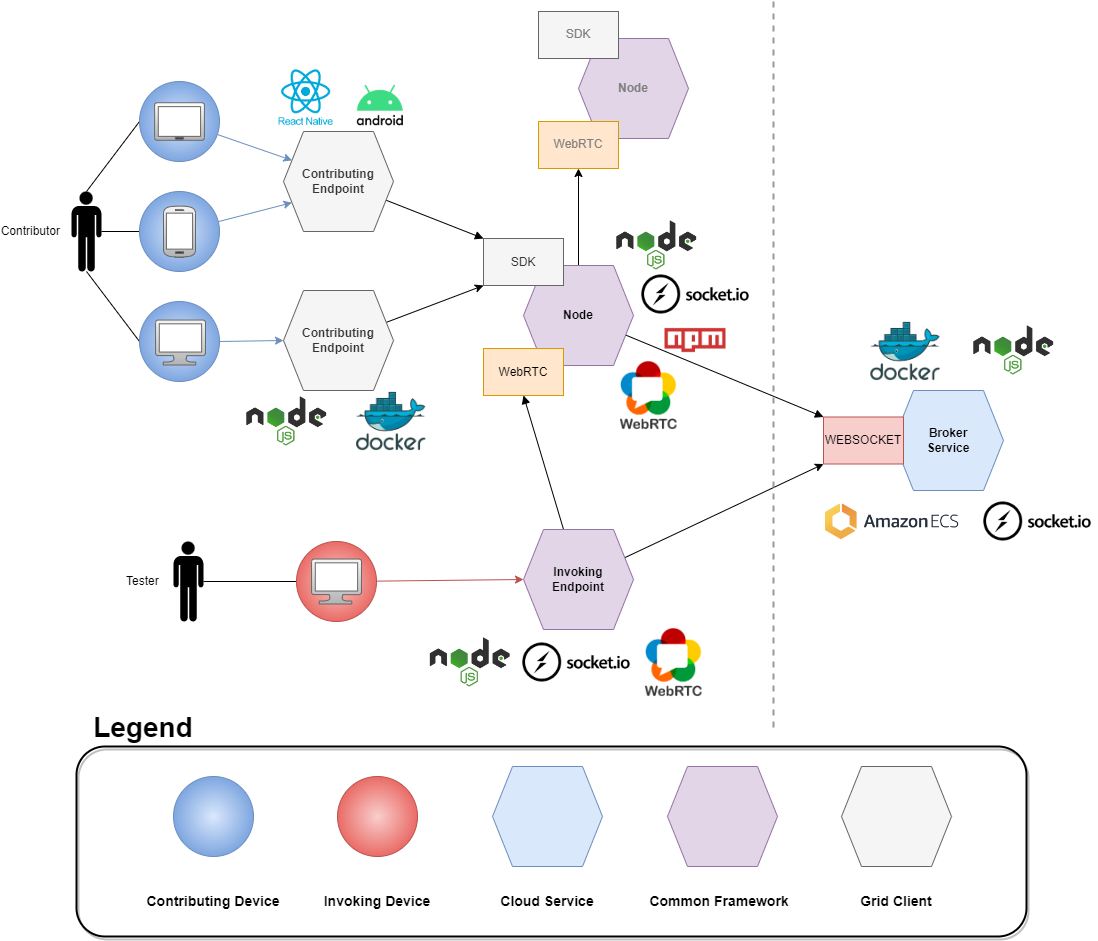
\includegraphics[width=\linewidth]{document/chapters/chapter_6/images/simplified_architecture.png}
    \caption{Complete view of the simplified prototype's architecture}
    \label{fig:simplified_architecture}
\end{figure}

\vspace{10mm}

\textbf{All the entities} composing the architecture \textbf{are implemented using technologies based on Node.js} which \textbf{offers useful, popular and well-maintained frameworks} as well as an \textbf{easy-to-use concurrency model based on an event loop}.

\subsection{Broker Service}
The \textbf{only Cloud Service} present in this simplified architecture is the \textbf{Broker Service}; since \textbf{only one instance} (with a static address) of such Cloud Service is required to sustain the workload of the few devices connected, \textbf{a dynamic handling and discovery of multiple instances is thus not required}. As a direct consequence of that, the complementary entities that handled the dynamic system for scalability (Grid Master Service, Broker Discovery Service and Grid Services Gateway Service) are not needed and thus \textbf{Nodes and Invoking Endpoints communicate directly with the Broker Service without first undergoing the discovery processes} described in \textit{section \ref{use_cases_satisfaction}}.

The prototype's Broker Service is implemented by using the \textbf{Typescript} language and utilizes \textbf{Socket.io} in order to create a web server that is reachable via WebSocket protocol; through the use of this technology, \textbf{Invoking Endpoints are able to deposit requests for the recruitment of Nodes that will be used to perform computations}. The messages involved in the recruiting process and the general Grid connection will be discussed in \textit{section \ref{coordination}}.

In order to have a running instance of the Broker Service that also has a static address reachable from anywhere, a \textbf{Docker image} is created which, in turn, is executed in a container through the use of \textbf{Amazon ECS} (Elastic Container Service). More details about the deployment of this entity will be discussed later in \textit{section \ref{devops}}.

\subsection{Interconnected Node}\label{interconnected_node}
The \textbf{Node} entity, which in the Interconnected project takes the name of \textbf{"\textit{Interconnected Node}"}, \textbf{contains all the logic regarding the contribution of a device}, and it is \textbf{distributed through NPM as a Node.js dependency} that is then \textbf{integrated in the concrete clients targeting various devices}.

Interconnected Node is also developed by using the \textbf{Typescript} language and, being this a client in the WebSocket connection to the Broker Service, it utilizes the client-side implementation of the \textbf{Socket.io} framework.

The \textbf{P2P connectivity} requirements are concretized through the use of the \textbf{WebRTC} (Real-Time Communication for the Web) protocol; such communication standard it is \textbf{used to send audio and video data among peers, as well as any kind of structured non-media data}. \textbf{In order for the peers to establish the connection, first the signaling process needs to be completed}: the Peers, through a third intermediary (the Broker Service), exchange some information required for the connection to happen; the Peer that initializes the connection creates an \textbf{SDP} (Signaling Description Protocol) object, denominated "\textbf{offer}". When the other Peer receives such data, it also creates its SDP object denominated "\textbf{answer}". Once each Peer possesses both generated SDP data, they finalize the connection exchanging some \textbf{ICE} (Interactive Connectivity Establishment) \textbf{candidates}; such ICE candidates need to be specified when realizing a WebRTC connection since they are the actual servers that allow the P2P connection. There are \textbf{two types of servers involved}:
\begin{itemize}
    \item \textbf{STUN} (Session Traversal Utilities for NAT)\\
    Used by Peers that reside behind the same NAT; through this server the IP info of each Peer are retrieved and a direct P2P connection can be established.
    \item \textbf{TURN} (Traversal Using Relays around NAT)\\
    Used by Peers that reside in different NATs; through this server the limitations of a NAT are overcome, creating an indirect P2P connection that uses the TURN server to forward the messages among the two Peers.
\end{itemize}

\begin{figure}[!ht]
    \centering
    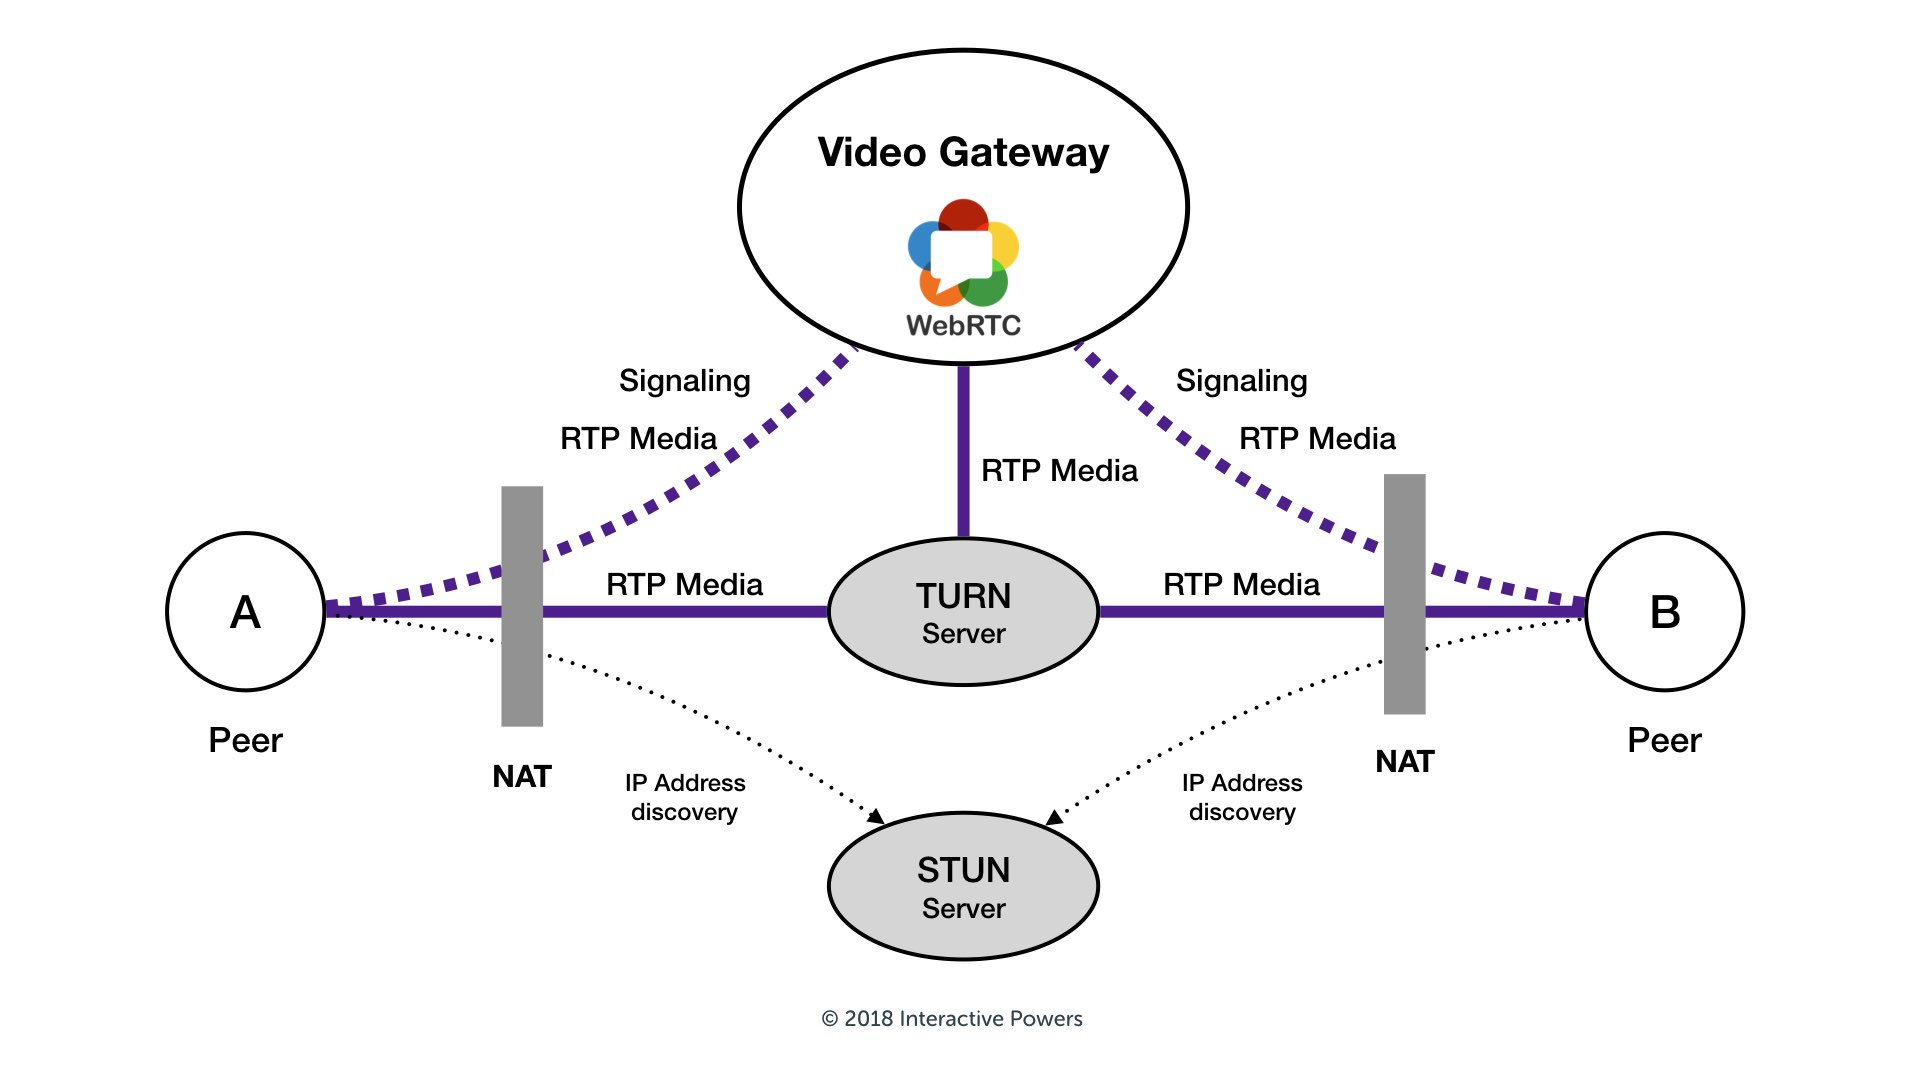
\includegraphics[scale=0.15]{document/chapters/chapter_6/images/webrtc.jpeg}
    \caption{WebRTC - STUN and TURN servers \cite{stun_and_turn_servers}}
    \label{fig:webrtc}
\end{figure}

Free STUN and TURN servers (used by this prototype) are available to the general public thanks to the \textbf{\href{https://www.metered.ca/tools/openrelay/}{Open Relay}} initiative.

There are both a \textbf{\href{https://www.npmjs.com/package/wrtc}{Desktop implementation}} and a \textbf{\href{https://www.npmjs.com/package/react-native-webrtc}{React Native implementation}} of Node.js modules that allow to perform P2P connections utilizing the WebRTC protocol but, despite functioning in the same way and exposing the same interfaces with identical methods, \textbf{the Desktop implementation does not work on React Native and vice versa}. In order to circumvent this problem, \textbf{the object handling the P2P connection is wrapped in an interface that needs to be concretized in the specific Desktop and Mobile implementations} (\textit{figure \ref{fig:p2p_wrapper}}); this also allows to \textbf{add some domain-specific logic}, assigning to the Peer that initializes the connection the "\textbf{Master}" role and the "\textbf{Slave}" role to the other Peer. 

\begin{figure}[!ht]
    \centering
    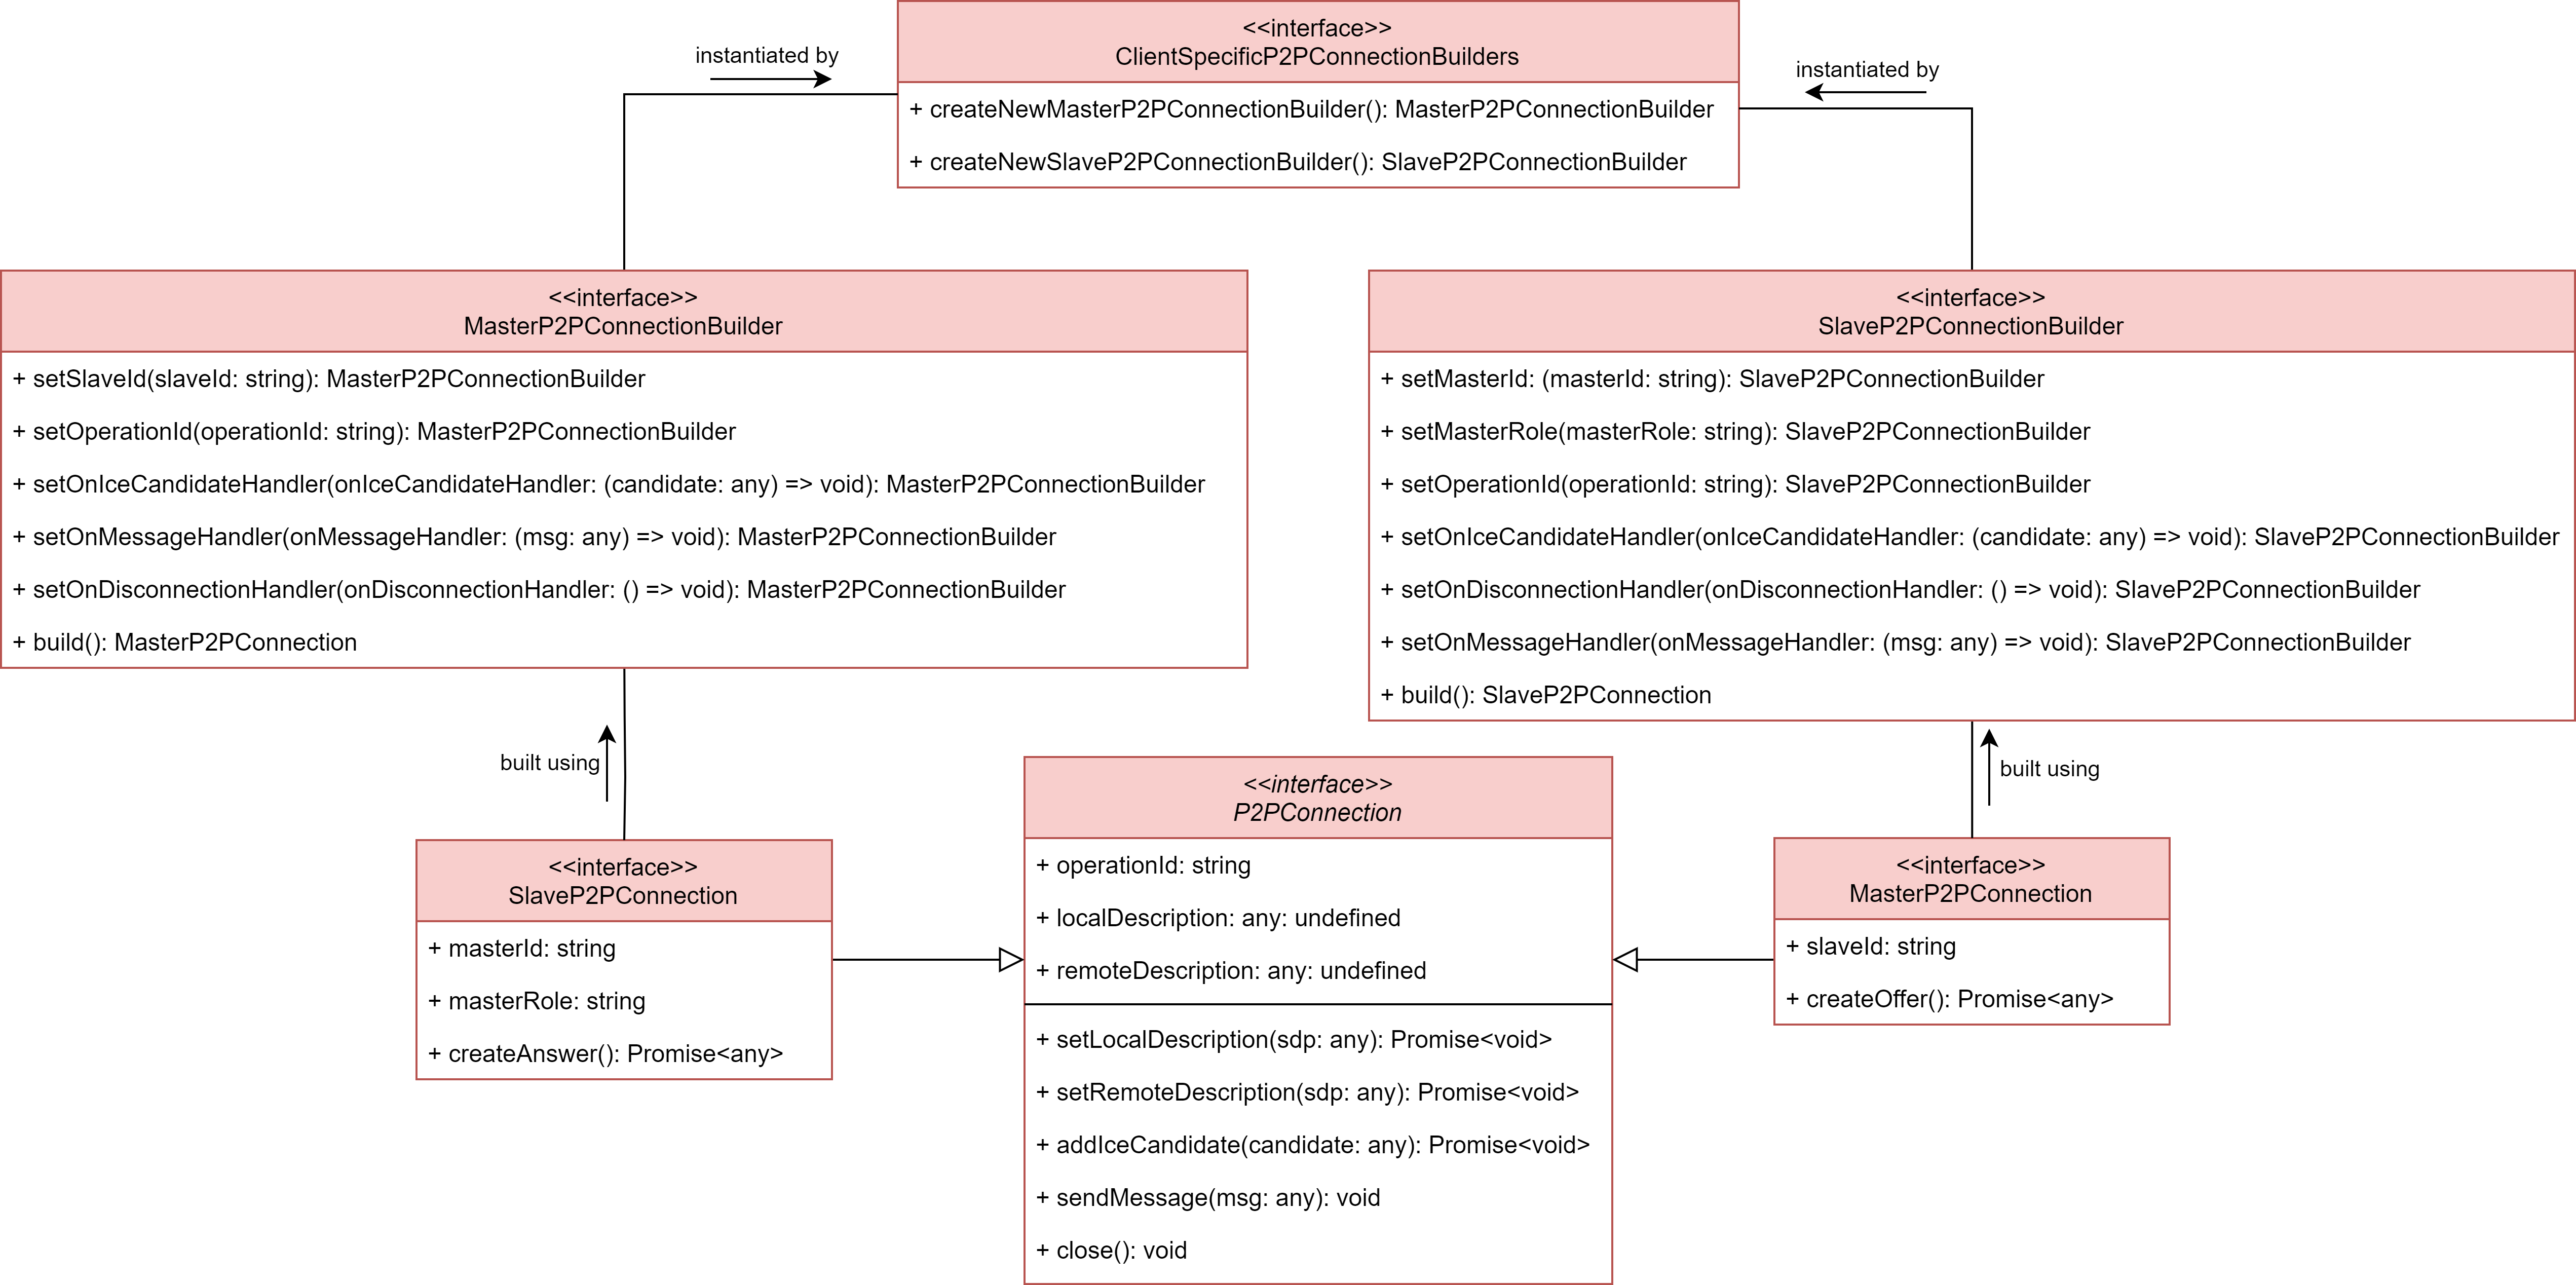
\includegraphics[width=\linewidth]{document/chapters/chapter_6/images/p2p_wrapper.png}
    \caption{WebRTC P2P Wrappers and builders}
    \label{fig:p2p_wrapper}
\end{figure}

\textbf{The construction of the client-specific objects is standardized through the utilization of the Builder pattern}, allowing the internal logic of the Interconnected Node to create instances of such objects without actually possessing the concrete implementation. \textbf{The P2P Builders} (along with a unique device identifier) \textbf{will then be passed at construction time to the InterconnectedNode Facade} (\textit{\ref{fig:interconnected_node_facade}}) \textbf{which exposes simple methods to interact with the core logic}, hiding its complexity and requiring the specific client only to deal with presentational aspects and device-specific responsibilities.

\begin{figure}[!ht]
    \centering
    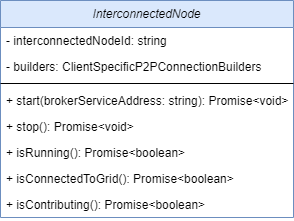
\includegraphics[scale=0.6]{document/chapters/chapter_6/images/interconnected_node_facade.png}
    \caption{Interconnected Node Facade}
    \label{fig:interconnected_node_facade}
\end{figure}

When it comes to the \textbf{actual computational contribution} that the Interconnected Node needs to perform, \textbf{two key abstractions are present}: \textbf{Job} and \textbf{Task}; a Job is an activity that a Slave Peer executes under the guidance of its Master that, after instructing the start of said Job, sends Tasks to execute in that specific Job.

\textbf{This abstraction results in the definition of common interfaces for Job and Task that are then concretized realizing new functionalities that will then be used to execute Grid Services} (MapReduceMasterJob, MapReduceMapWorkerJob, etc...); through this mechanism, expanding the support for new Grid Services only requires to define new concrete Jobs and Tasks, realizing their logic and their handlers for the messages exchanged among Nodes.

\subsection{Interconnected Mobile Client}
In this prototype, the \textbf{mobile incarnation of the Contributing Endpoint} takes the name of \textbf{"Interconnected Mobile Client"}. The main technology used for realizing this client is \textbf{React Native} (which is also \textbf{Node.js based}); with this framework, it is possible to \textbf{build mobile applications targeting both Android and iOS devices with just one code base} while also \textbf{taking advantage of most of the modules available on NPM}.

Thanks to this Node.js compatibility, \textbf{the mobile client is able to use the Interconnected Node to connect to the Grid and perform contributions, only requiring to implement previously mentioned client-specific interfaces and to provide an ID for the device} (given the limited number of devices in the prototype setting, a \textbf{UUID v4} is generated and used as the ID).

Although React Native also allows targeting iOS devices, \textbf{this prototype is tested only on Android devices}; this limitation is caused by the previously mentioned lack of resources (in particular the unavailability of Apple devices to test it on) but, in theory, the application should also function on iPhones and iPads with little to no changes to the code base.

\vspace{10mm}

\begin{figure}[!ht]
    \centering
    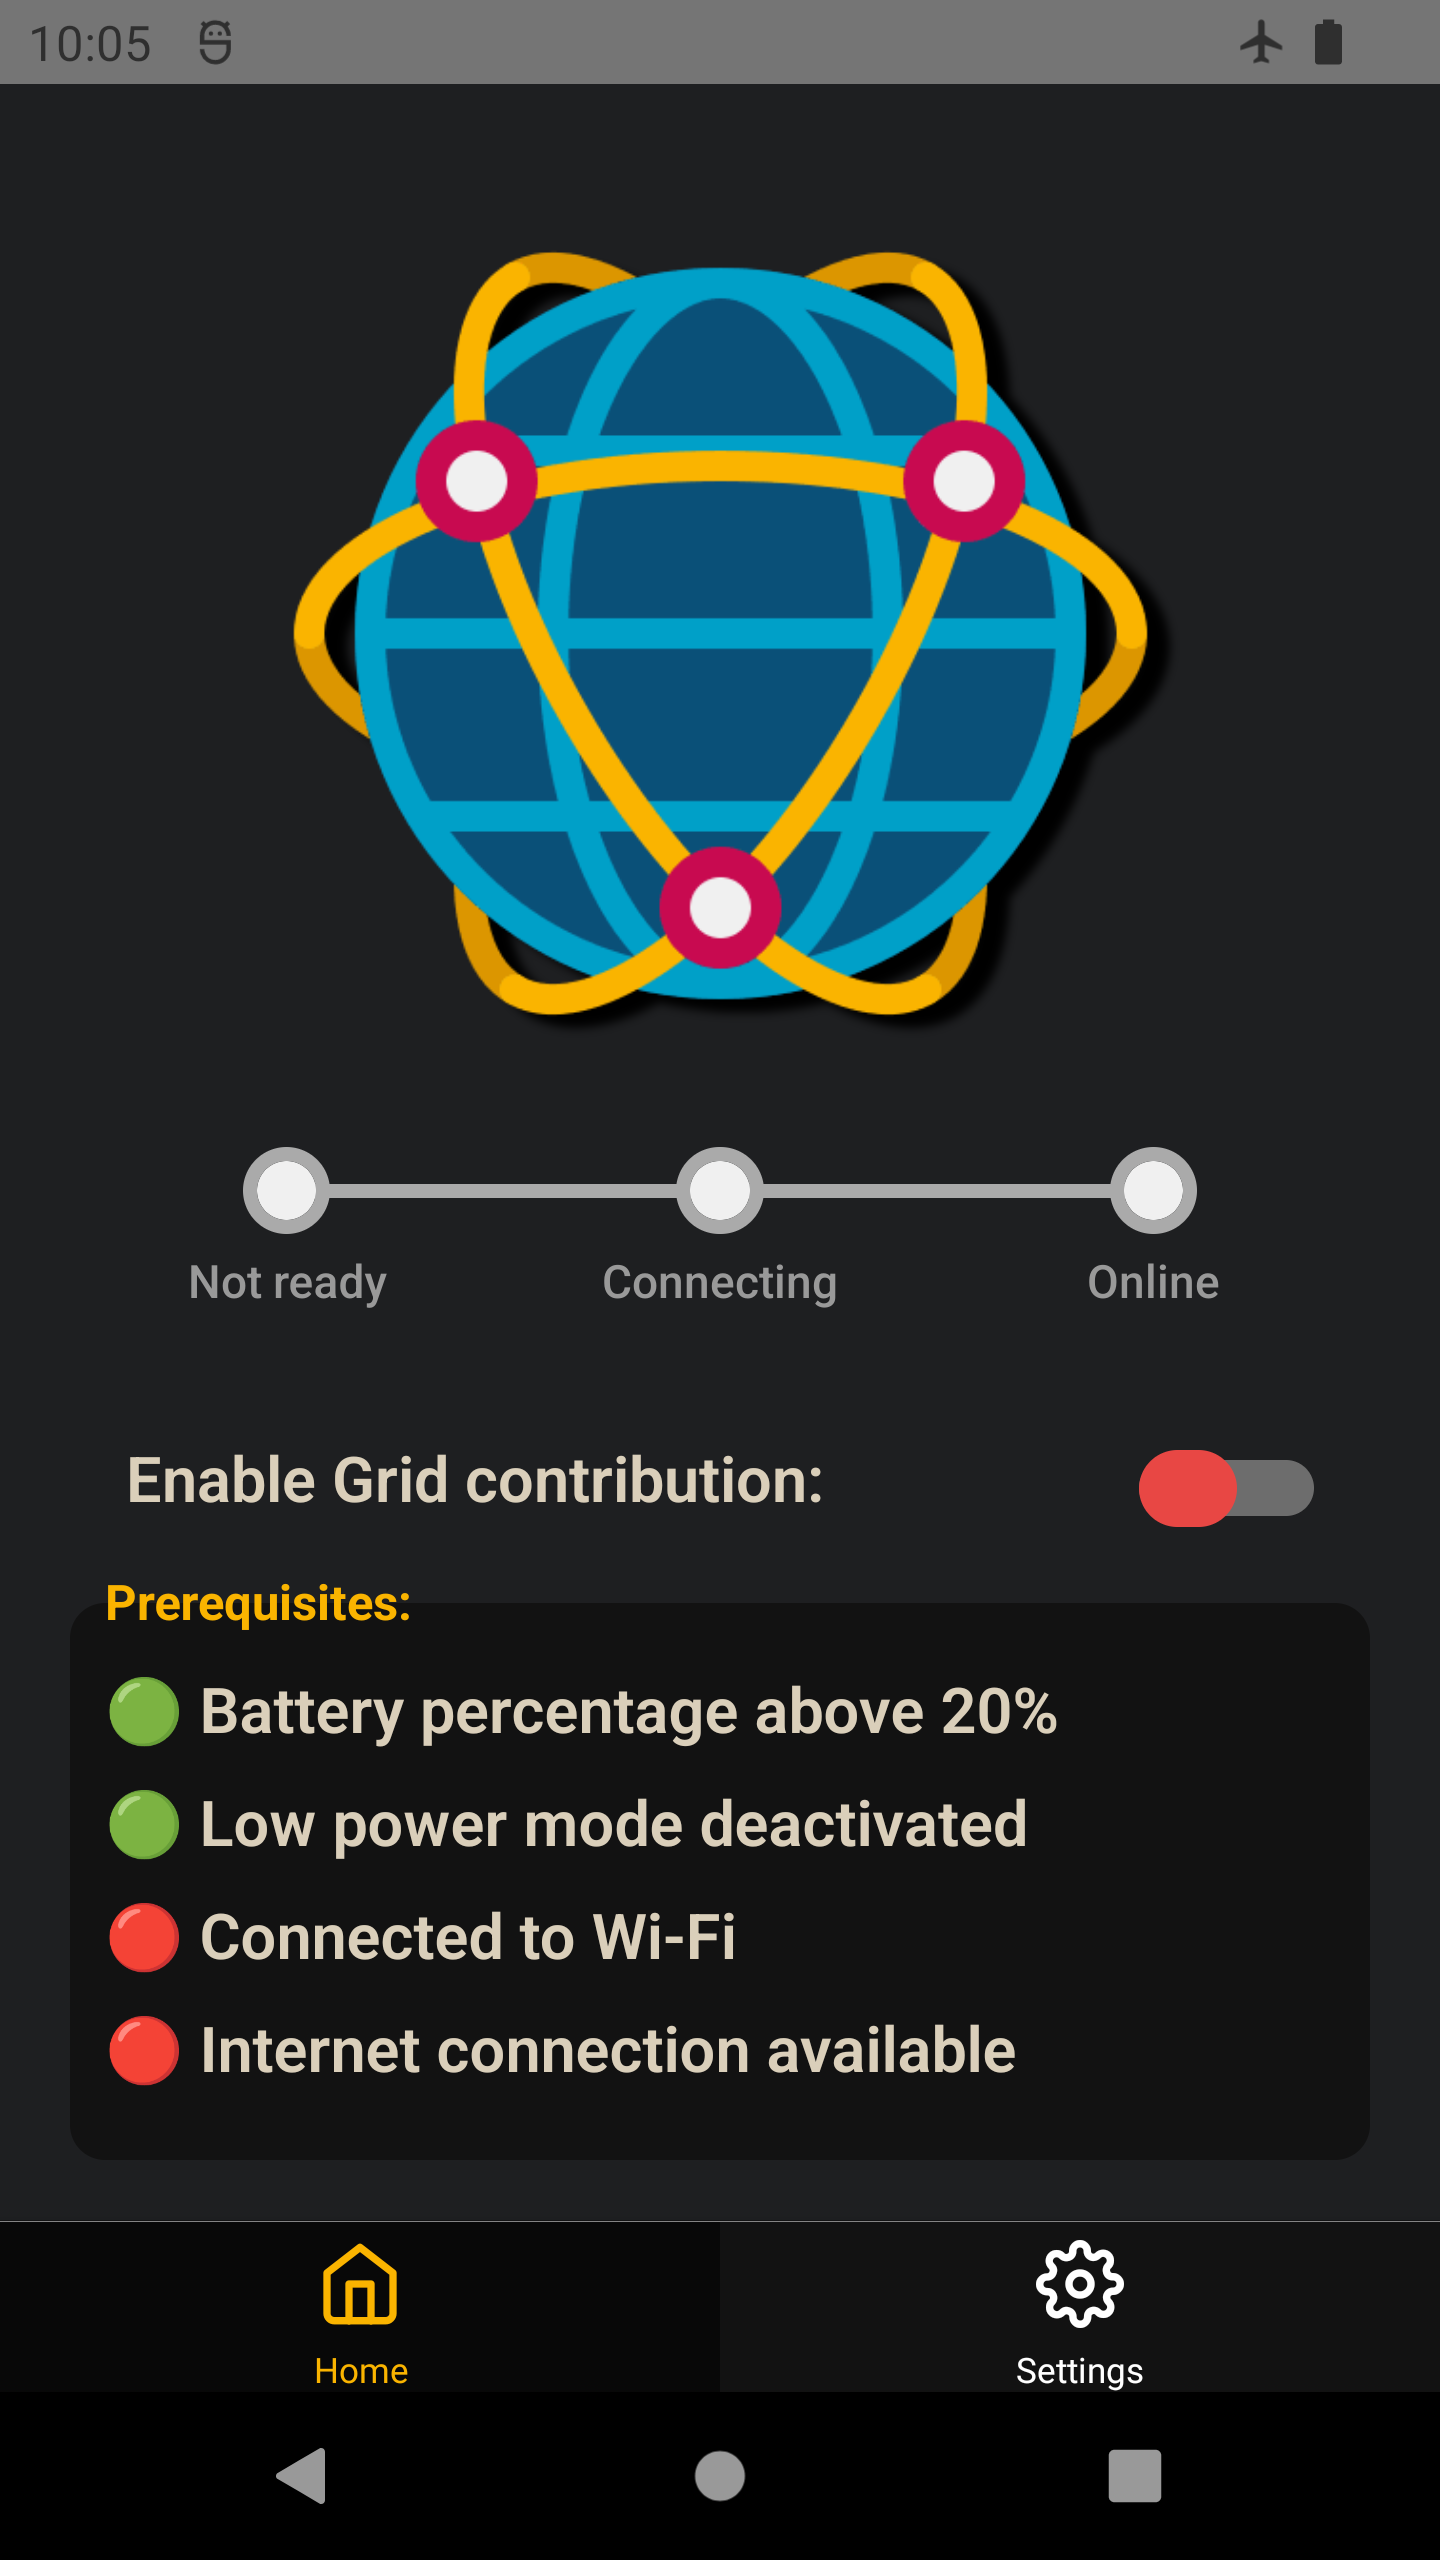
\includegraphics[scale=0.12]{document/chapters/chapter_6/images/interconnected_mobile_home.png}
    \caption{Interconnected Mobile Client}
    \label{fig:interconnected_mobile_home}
\end{figure}

\textit{Figure \ref{fig:interconnected_mobile_home}} shows the \textbf{GUI} of the application: \textbf{by simply activating the "Enable Grid contribution" switch} (\textit{figure \ref{fig:interconnected_mobile_connection}(a)}), \textbf{the application starts a background process that continues to operate even after the application is closed}; Android forces the developer to notify the user of the presence of a \textbf{background activity} by spawning a \textbf{permanent notification} (which can be seen in \textit{figure \ref{fig:notification_contribution}}) that will automatically be removed when the background activity is stopped by disabling the switch.

This background process is responsible for checking a series of conditions (that are listed in the \textbf{"Prerequisites"} section of the GUI) which are necessary for Grid Contribution; \textbf{when all the conditions are met, the Interconnected Node is started through the use of the previously mentioned Facade} exposed by the module. \textbf{In case even one of the prerequisites is not satisfied anymore, the Interconnected Node is stopped}.

\begin{figure}[!ht]
    \centering
    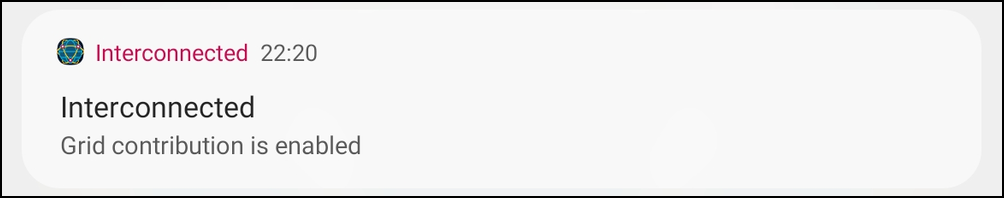
\includegraphics[scale=0.35]{document/chapters/chapter_6/images/notification_contribution.png}
    \caption{Interconnected Mobile Client - Grid contribution enabled notification}
    \label{fig:notification_contribution}
\end{figure}

\begin{figure}[!ht]
    \centering
    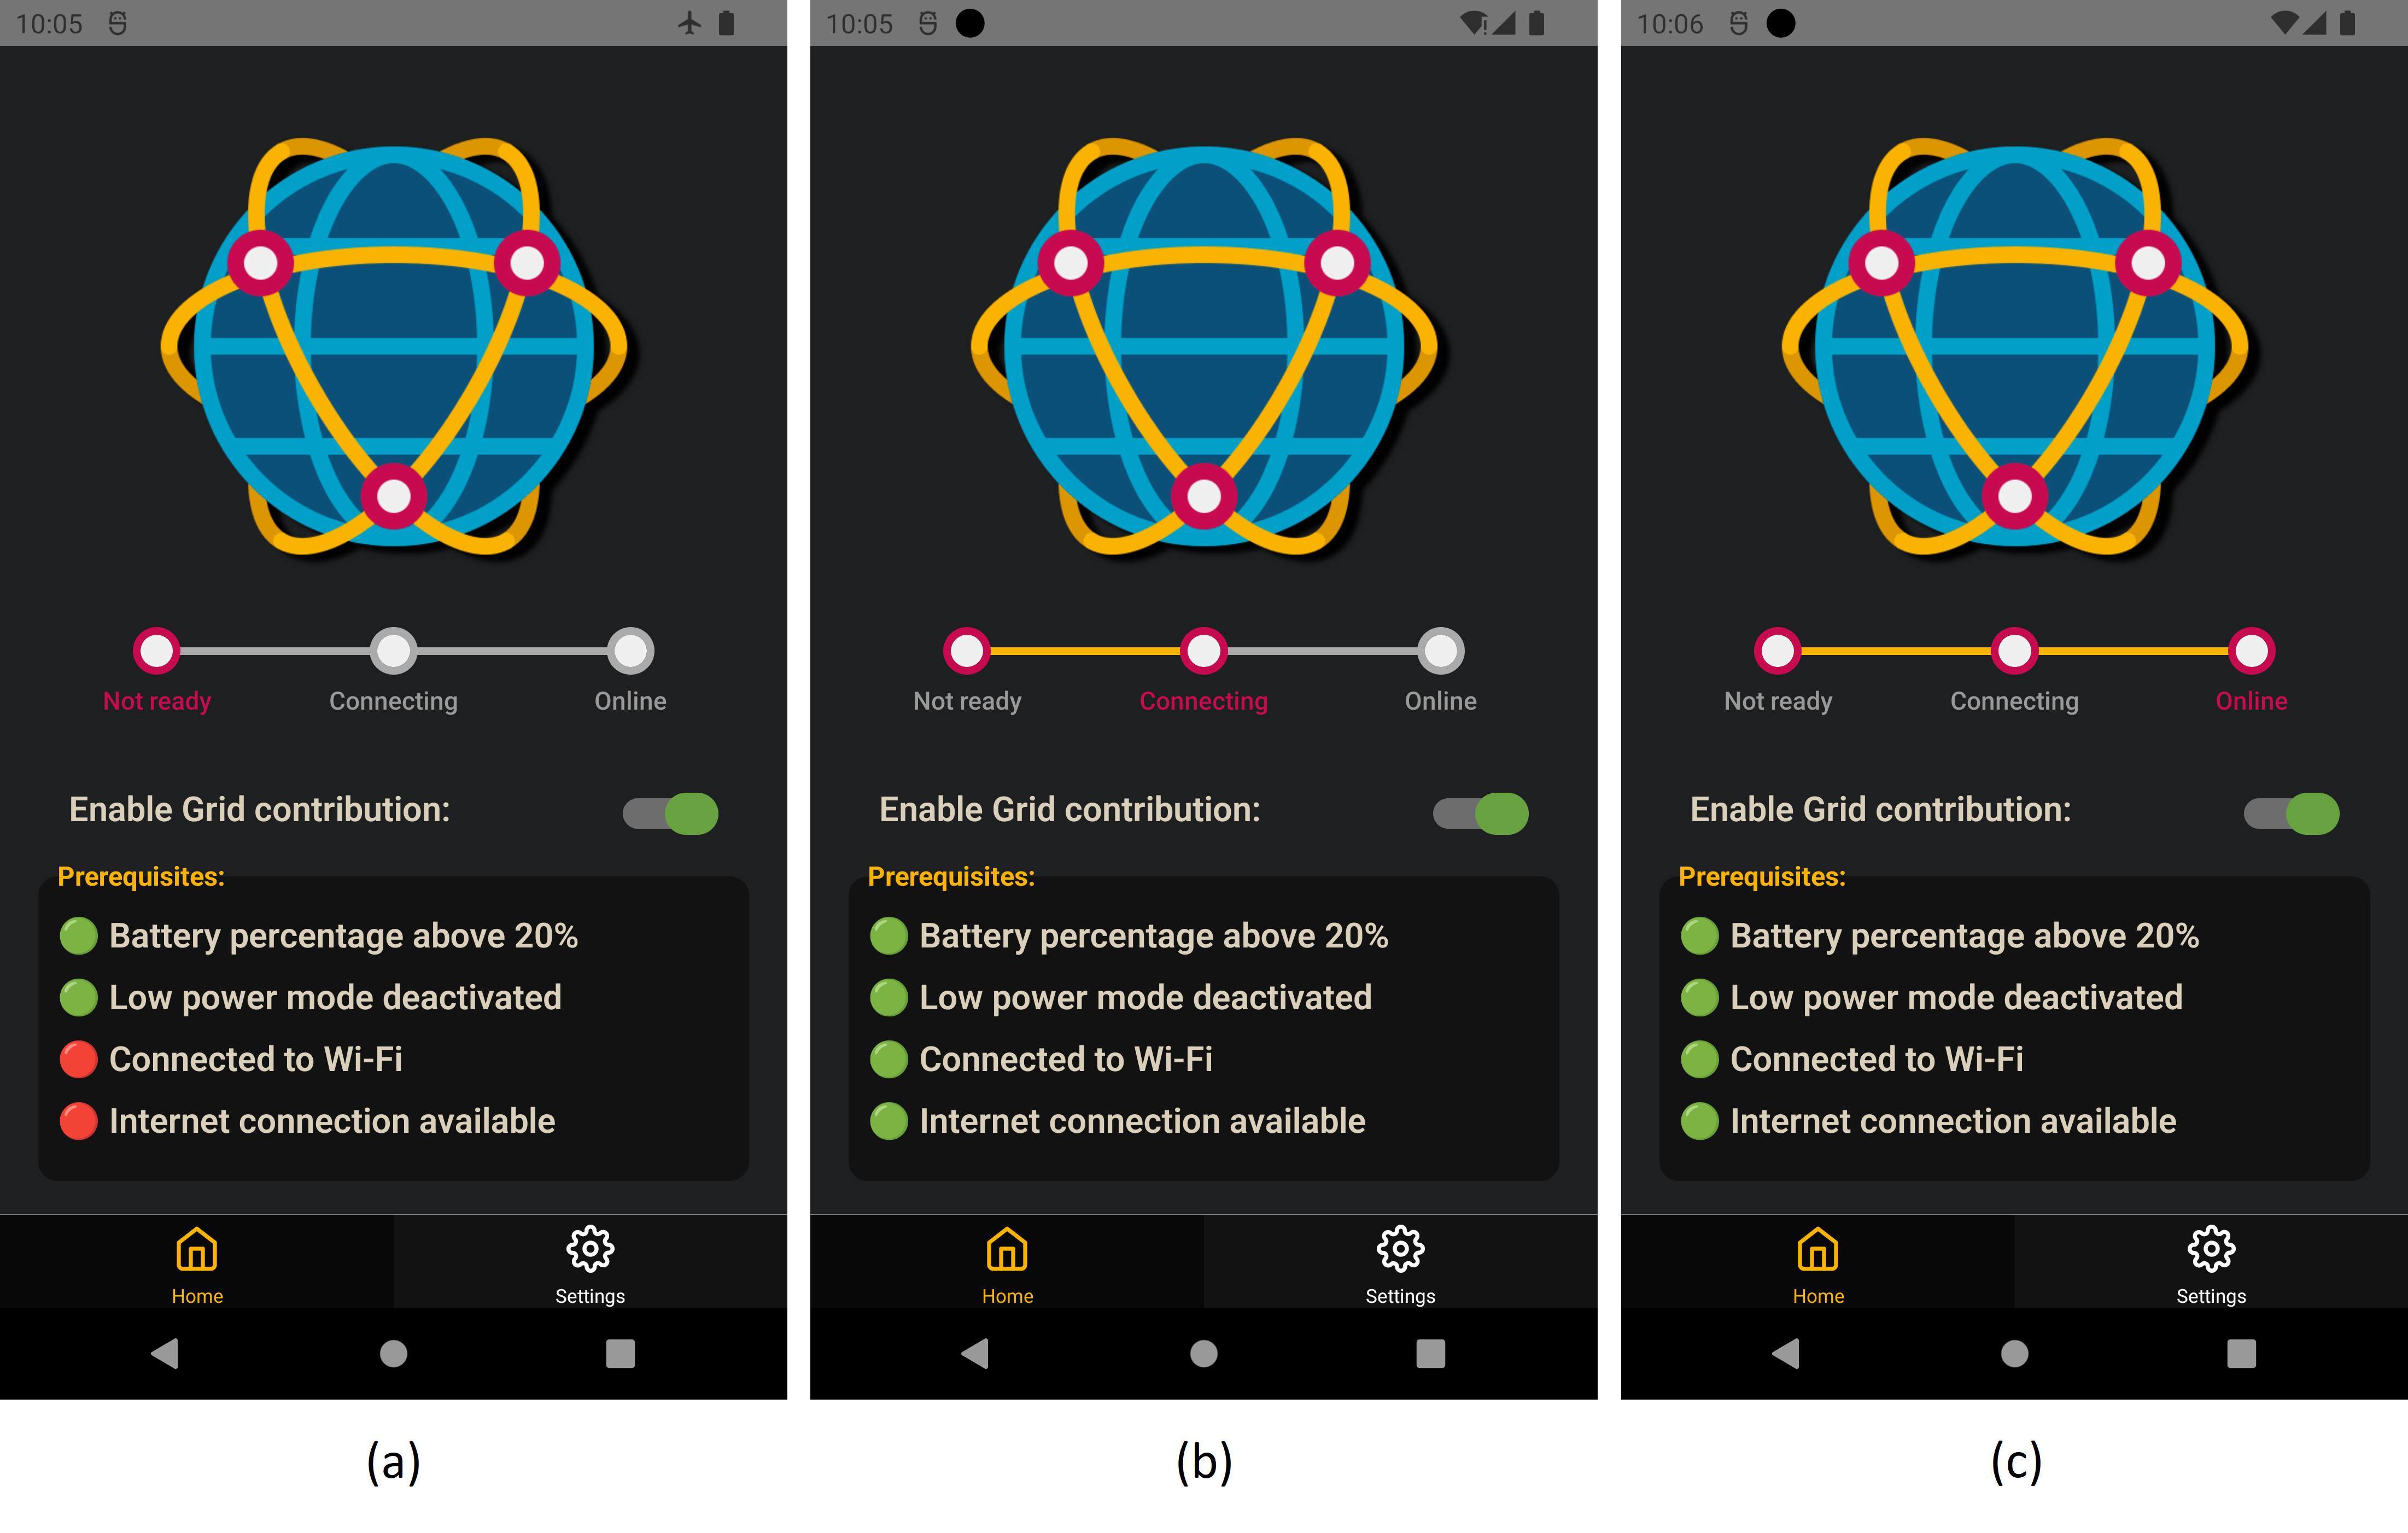
\includegraphics[width=\linewidth]{document/chapters/chapter_6/images/interconnected_mobile_connection.png}
    \caption{Interconnected Mobile Client - Status}
    \label{fig:interconnected_mobile_connection}
\end{figure}

Despite being a background process, \textbf{the user can check the application's status through the GUI's indicators}: after the activation of the background process, the application remains in the \textbf{"Not ready"} state until all the Prerequisites are met (becoming green); after that, there is a transition to the \textbf{"Connecting"} state (\textit{figure \ref{fig:interconnected_mobile_connection}(b)}) and, once the Grid Connection is established, the \textbf{"Online"} state is reached (\textit{figure \ref{fig:interconnected_mobile_connection}(c)}).

\textbf{When a contribution to a Grid Service is currently being performed, the user is notified by a notification} that, once the contribution is over, is then updated showing that the process is complete (\textit{figure \ref{fig:notification_completed}}).

\begin{figure}[!ht]
    \centering
    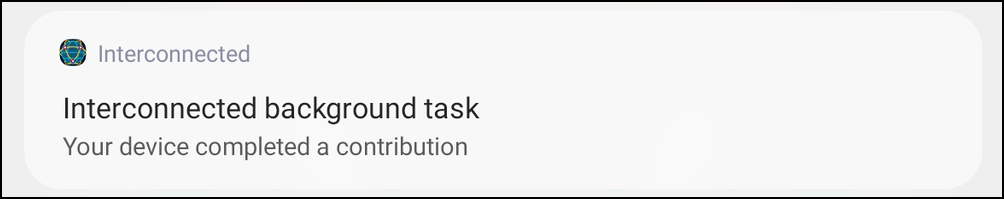
\includegraphics[scale=0.35]{document/chapters/chapter_6/images/notification_completed.png}
    \caption{Interconnected Mobile Client - Grid contribution completed notification}
    \label{fig:notification_completed}
\end{figure}

\subsection{Interconnected Desktop Client}
The \textbf{Desktop incarnation of the Contributing Endpoint} takes the name of \textbf{"\textit{Interconnected Desktop Client}"}; like the Mobile counterpart, it is developed using the \textbf{Typescript} language and by \textbf{relying on the Interconnected Node module dependency}. For this prototype version \textbf{no GUI was developed} and, then, a simple \textbf{Docker image} (which can run on any computer) is provided.

\begin{figure}[!ht]
    \centering
    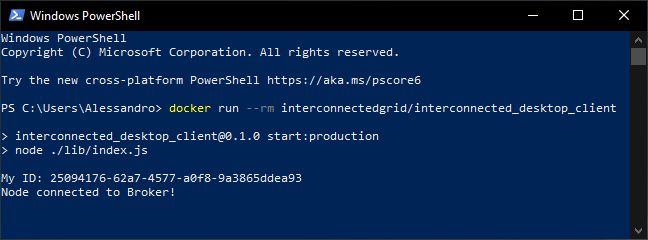
\includegraphics[scale=0.8]{document/chapters/chapter_6/images/interconnected_desktop.png}
    \caption{Interconnected Desktop Client - Docker image run on a container}
    \label{fig:interconnected_desktop}
\end{figure}

In the Interconnected Mobile Client, this prototype's \textbf{Node ID} is generated by using a simple \textbf{UUID v4} (which can be seen in \textit{figure \ref{fig:interconnected_desktop}}).

\subsection{Invoking Endpoint Prototype}
The last entity that composes this simplified architecture is the \textbf{\textit{Invoking Endpoint Prototype}}; unlike its counterpart in the complete architecture, which envisions it as a dependency (much like the Interconnected Node) that can be used by a Customer Custom application, this prototype version is a \textbf{standalone program that can interact with the Grid launching a MapReduce computation}; more details on the subject will be discussed in \textit{section \ref{real_world_experiments}}.

This entity is developed, like the others, relaying on the \textbf{Node.js framework} but, instead, by using plain \textbf{JavaScript} and not the Typescript superset. In order to be able to communicate with the Broker Service and the Interconnected Nodes, it also utilizes the \textbf{Socket.io} module and the \textbf{WebRTC module}, respectively.
\section{DevOps}\label{devops}
The project utilizes a series of services to facilitate the production cycle, starting from version control combined with automation that simplifies the release process.

\textbf{GitHub} was chosen as the primary hub for the code base. In particular the \textbf{"GitHub organizations"} feature of such service allows creating organizations where people can cooperate and, most importantly, it groups together repositories belonging to that specific organization, separating them from personal accounts.

\begin{figure}[!ht]
    \centering
    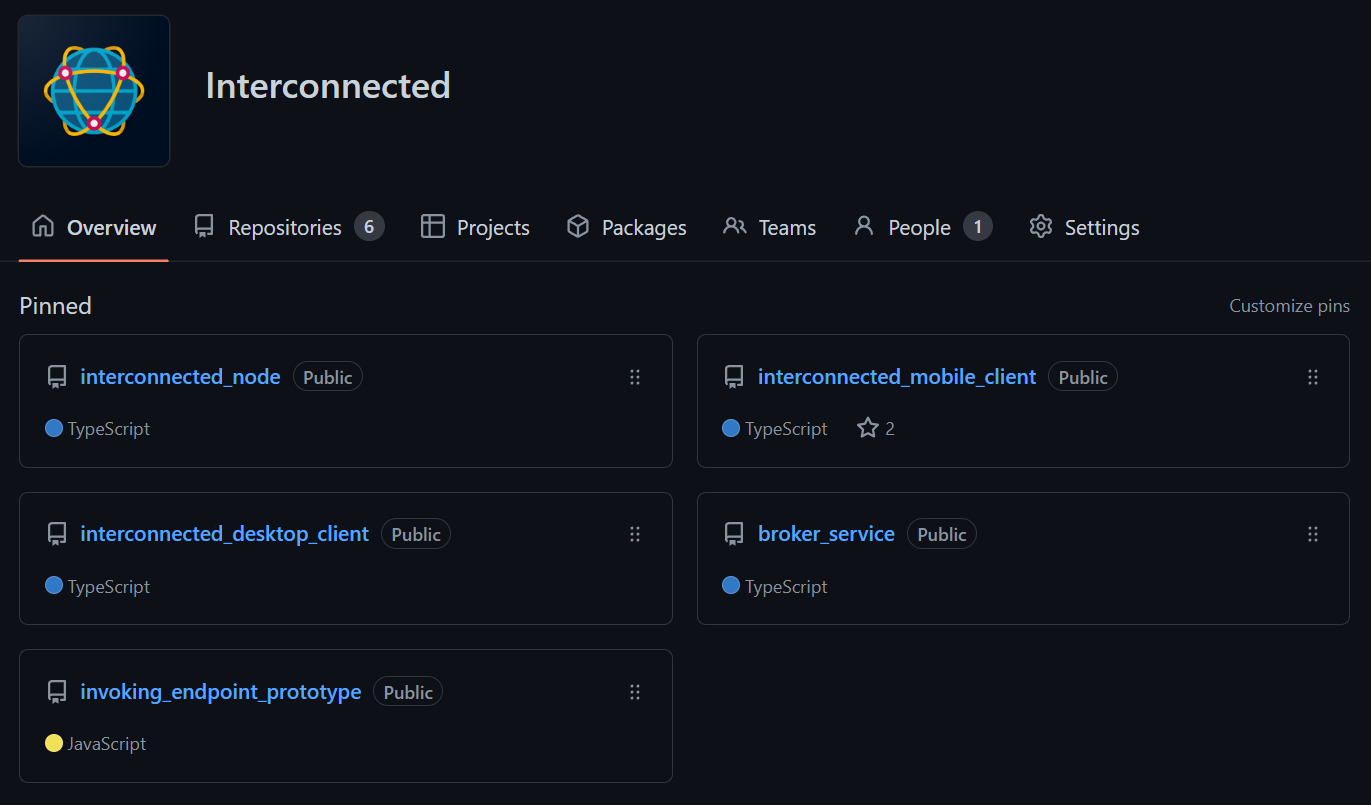
\includegraphics[width=\linewidth]{document/chapters/chapter_6/images/interconnected_organization.png}
    \caption{Interconnected - \href{https://github.com/Interconnected-project}{GitHub Organization}}
    \label{fig:interconnected_organization}
\end{figure}

Furthermore, through the definition of specific \textbf{GitHub actions}, a lot of repetitive tasks can be automated; in this project case, actions collaborate with external services in order to obtain \textbf{CD} (Continuous Delivery) \textbf{automation}.

The first external service used is \textbf{NPM}; \textbf{when a new release of the Interconnected Node is created, a GitHub action uses the repository's code base in order to publish the module on NPM} (\textit{figure \ref{fig:interconnected_npm}}), making it available for the Mobile and Desktop Contributing Endpoints.

\begin{figure}[!ht]
    \centering
    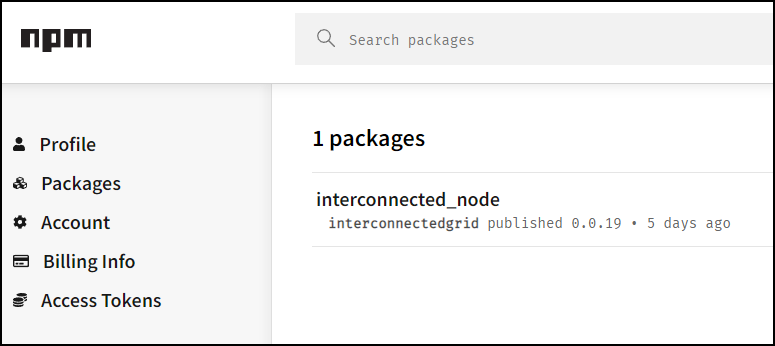
\includegraphics[scale=0.45]{document/chapters/chapter_6/images/interconnected_npm.png}
    \caption{Interconnected - \href{https://www.npmjs.com/package/interconnected_node}{NPM}}
    \label{fig:interconnected_npm}
\end{figure}

The Broker Service and the Interconnected Desktop Client both utilize Docker for the execution on target machines; such \textbf{Docker images are automatically created and published on Docker Hub whenever a new release is created in the respective repositories}. Thanks to this, a machine that wants to run a container with that specific image will not need to access the code base and run, compile and run the Node.js environment, but it will only need a working installation of the Docker client; knowing the image name, this will automatically be downloaded from Docker Hub to the target machine (\textit{figure \ref{fig:interconnected_desktop}}). 

\begin{figure}[!ht]
    \centering
    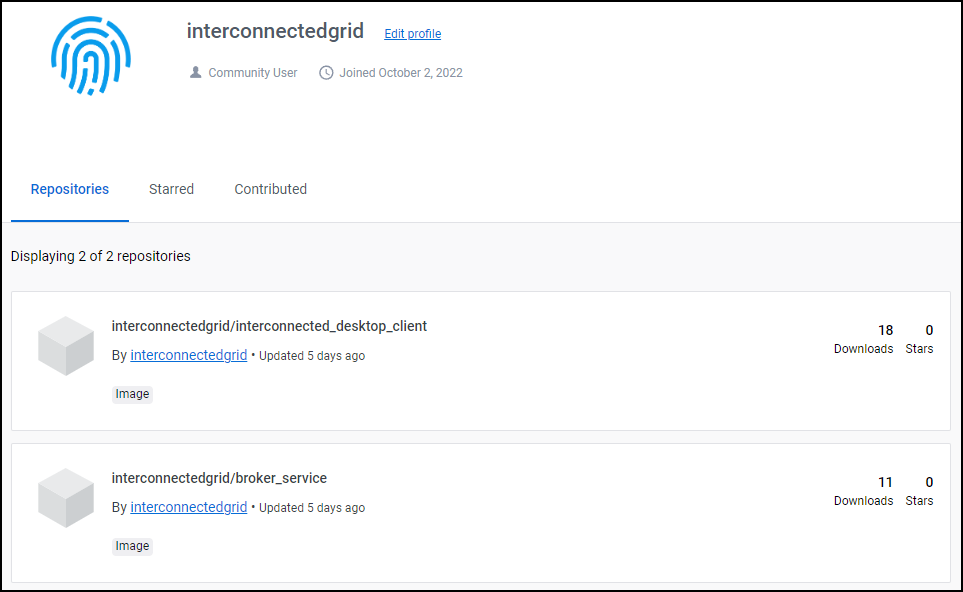
\includegraphics[width=\linewidth]{document/chapters/chapter_6/images/interconnected_dockerhub.png}
    \caption{Interconnected - \href{https://hub.docker.com/u/interconnectedgrid}{Docker Hub}}
    \label{fig:interconnected_dockerhub}
\end{figure}

In particular, when it comes to the execution of the Broker Service's image on a container, Amazon ECS offers a simple hosting platform that is able to pull images from Docker Hub by simply defining a task and running it. This way, \textbf{every time the Broker Service is started, Amazon ECS' defined task will retrieve the latest published image and will run it on a dedicated container} (\textit{figure \ref{fig:interconnected_ecs}}).

\begin{figure}[!ht]
    \centering
    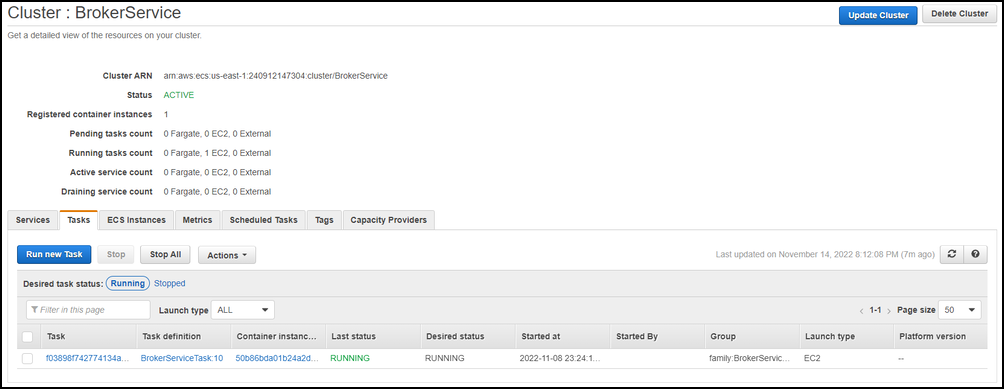
\includegraphics[scale=0.37]{document/chapters/chapter_6/images/interconnected_ecs.png}
    \caption{Interconnected - Amazon ECS}
    \label{fig:interconnected_ecs}
\end{figure}

Finally, despite being run on an emulator during development, the \textbf{Interconnected Mobile Client} needs to be delivered in production; \textbf{each time a new release is created on its GitHub repository, an action will build an APK and publish it as an attached file to said release}. This way, a ready-to-use installer is automatically made available for installation on real Android devices.

\begin{figure}[!ht]
    \centering
    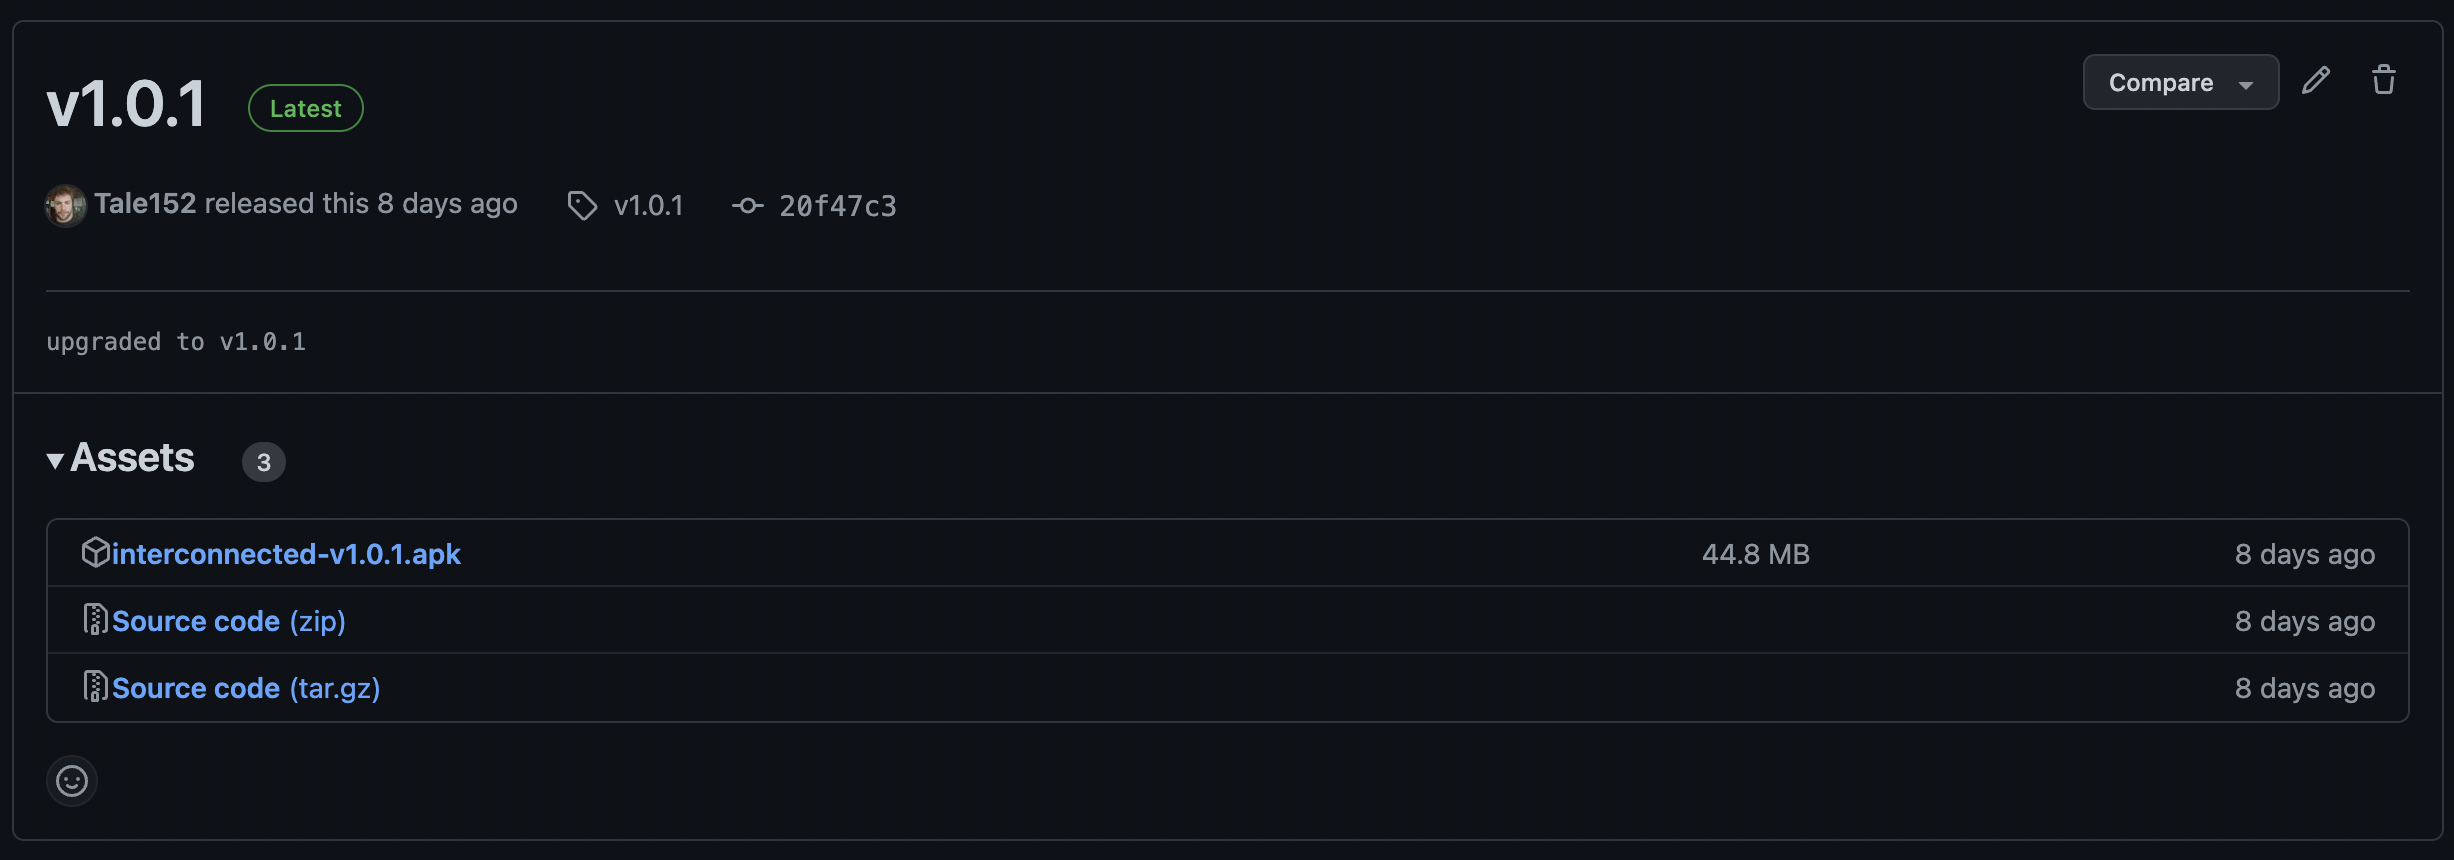
\includegraphics[scale=0.3]{document/chapters/chapter_6/images/github_actions_apk.png}
    \caption{Interconnected - \href{https://github.com/Interconnected-project/interconnected_mobile_client/releases}{Android APK automated release}}
    \label{fig:github_actions_apk}
\end{figure}
\section{Coordination}\label{coordination}
This section analyses the \textbf{messages exchanged among the entities composing the prototype architecture}. There are \textbf{three phases} in this coordination process:
\begin{enumerate}
    \item \textbf{Grid connection}
    \item \textbf{Recruitment}
    \item \textbf{P2P messaging}
\end{enumerate}

\subsection{Grid connection}
This phase \textbf{connects a Node} (whether used by the Mobile or the Desktop client) \textbf{or an Invoking Endpoint Prototype to the Broker Service using a Socket connection} through the Socket.io framework. \textbf{The Broker Service registers the connections and uses them in the Recruitment phase}.

\subsection{Recruitment}
The recruitment phase \textbf{connects a requestor device} (that becomes the Master in the P2Pconnection) \textbf{to an actual device that will perform a Contribution} (becoming the Slave). \textbf{While a Slave is necessarily a Node, a Master can either be an Invoking Endpoint or a Node}, allowing to obtain either an \textbf{Invoking Endpoint to Node connection} or a \textbf{Node to Node connection}.

This phase is \textbf{executed exchanging messages among the soon-to-be Peers using the previously established Socket connections, but ends with a direct P2P connection} between the Master and the Slave through the WebRTC framework.

\begin{figure}[!ht]
    \centering
    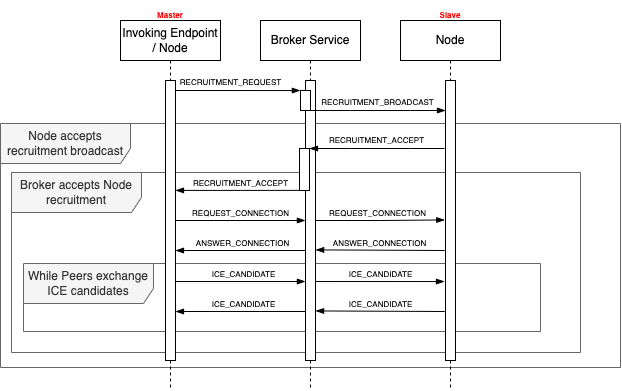
\includegraphics[scale=0.65]{document/chapters/chapter_6/images/recruitment_messages.png}
    \caption{Recruitment - Sequence Diagram}
    \label{fig:recruitment_messages}
\end{figure}

\textit{Figure \ref{fig:recruitment_messages}} shows the actual messages exchanged in this phase: the soon-to-be Master sends a \textbf{\textit{RECRUITMENT\_REQUEST}} to the Broker Service, \textbf{containing details regarding which kind of resources are needed}; the Broker Service, upon receiving this request, creates a \textbf{pending Recruitment Request} and broadcasts a \textbf{\textit{RECRUITMENT\_BROADCAST}} message to all the connected Nodes.

\textbf{The Node checks locally if it is compatible with the received request} and, if all the conditions are true, it sends a \textit{\textbf{RECRUITMENT\_ACCEPT}} message \textbf{to the Broker Service} which, upon receiving it, checks if the request is still unsatisfied, \textbf{eventually forwarding the message to the entity that first emitted the request}.

From this point on, \textbf{the P2P connection is initialized exchanging the WebRTC's required information} (previously discussed in \textit{section \ref{interconnected_node}}): the \textbf{Master} sends a \textbf{\textit{REQUEST\_CONNECTION}} message, containing its \textbf{SPD offer} and, in response, the \textbf{Slave} sends its \textbf{SDP answer} contained in a \textbf{\textit{ANSWER\_CONNECTION}} message. Once the two Peers possess each other's SDP data structures, they \textbf{start exchanging ICE candidates until they reach an agreement, finally opening the P2P connection, completing the Recruitment}.

Although the broadcast is executed once, the messages contained in the "Broker accepts Node recruitment" scope need to be exchanged every time a new P2P connection is established among two Peers.

\subsection{P2P messaging}
\textbf{Once the P2P connection is established}, \textit{figure \ref{fig:p2p_messages}} shows the \textbf{messages that the Master and the Slave exchange in their interaction}.

\begin{figure}[!ht]
    \centering
    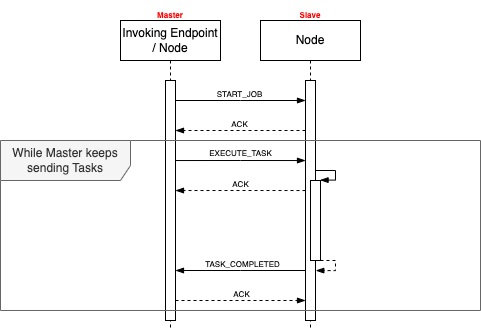
\includegraphics[scale=0.61]{document/chapters/chapter_6/images/p2p_messages.png}
    \caption{P2P messaging - Sequence Diagram}
    \label{fig:p2p_messages}
\end{figure}

\textbf{The Master sends a \textit{START\_JOB} message to the Slave}, possibly including data (which need to be sent only once) that will later be useful when executing the specific Tasks for that Job. Once the Slave has started said Job, t\textbf{he Master sends a \textbf{EXECUTE\_TASK} message}, \textbf{containing further data that}, combined with the Job's payload, \textbf{is used to perform a computation}. Upon receiving the EXECUTE\_TASK message the \textbf{Slave} sends an ACK to the Master and \textbf{enqueues the Task}, sending a \textbf{\textbf{TASK\_COMPLETED}} message (containing the result) to the Master \textbf{only when the task is actually completed}.

\textbf{This asynchronous organization allows the Master to send multiple Tasks to enqueue without waiting that the Slave has already completed its Tasks, speeding up the process}.
The Tasks submission and collection of results continues until all the Master's Tasks are completed and the P2P connection is terminated, removing the Job from the Slave.

\textbf{Using this Job/Task generalization, it is possible to construct various kinds of Grid Services}, starting from the MapReduce one.
\section{Proto-MapReduce}
\textbf{The MapReduce implementation used in this prototype is a simplified version} of what discussed in \textit{appendix \ref{the_mapreduce_paradigm}}; said simplifications, while making it \textbf{easier to implement}, have the \textbf{side effect of negatively influencing performances but}, given the available time limitations, they are \textbf{still acceptable in a prototypical context where the focus is to demonstrate the feasibility of mobile devices Contribution}.

\textbf{The first difference comes from how the data are handled}. The MapReduce paradigms handles a number of splits M and applies progressively the Map function to said splits; the intermediate results are grouped by key (using a partitioning function) in order to obtain R (with R<M, typically) partitions which, upon allying the Reduce function, will produce R final results. This \textbf{simplified version}, on the contrary, \textbf{takes the M splits} and, after applying the Map function, \textbf{maintains the original grouping, producing M intermediate results}; said results are then \textbf{computed applying the Reduce function} to each of them, \textbf{producing the M final results}. As a consequence, \textbf{the number of input data regions is equal to the regions in the final results}.

\vspace{10mm}

\begin{figure}[!ht]
    \centering
    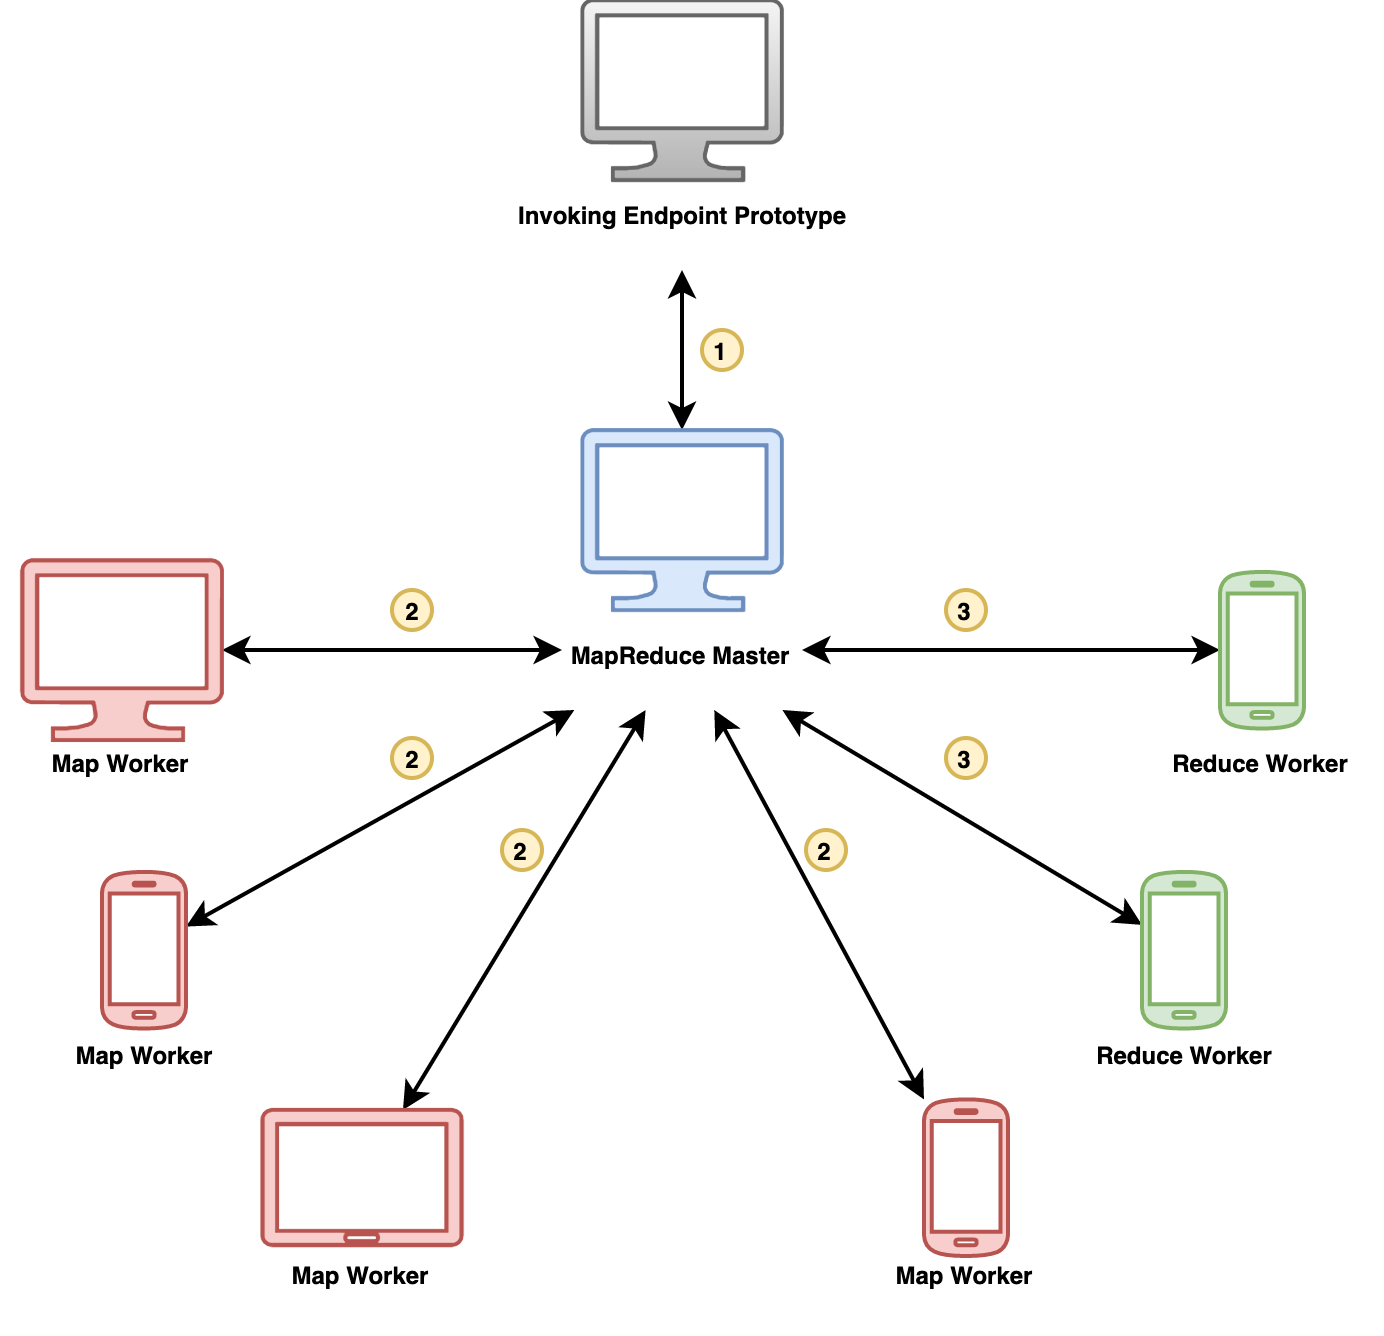
\includegraphics[scale=1]{document/chapters/chapter_6/images/proto_mapreduce.png}
    \caption{Proto-MapReduce Topology}
    \label{fig:proto_mapreduce}
\end{figure}

\textbf{The second important distinction comes from the topology of the connections among the entities involved} in the MapReduce operation. Normally, a Map Worker that has completed a run of the Map function would send, under the coordination of the MapReduce Master, its intermediate results directly to the right Reduce worker; \textbf{in this simplified version a Map Worker that has completed a Map operation sends its results to the MapReduce Master which, after gathering all the Map results for that particular region, will forward the data to an assigned Reduce Worker}. The final topology for the MapReduce Service performed in this prototype is shown in \textit{figure \ref{fig:proto_mapreduce}} and is \textbf{obtained performing these three steps}:
\begin{enumerate}
    \item \textbf{MapReduce Master recruitment}\\
    The Invoking Endpoint Prototype performs a recruitment (seen in \textit{figure \ref{fig:recruitment_messages}}), connecting to a Node which receives a MapReduce Master Job (containing all info about resources requested with the Map and Reduce functions definitions as well). This marks the beginning of the next phase but, in the meantime, the Invoking Endpoint starts sending Tasks to the MapReduce Master (\textit{figure \ref{fig:p2p_messages}}), each containing a data region to compute.
    \item \textbf{Map Workers recruitment}\\
    The MapReduce Master performs a recruitment, requesting the Map Workers specified in its MapReduce Master Job, and it sends a Map Worker Job (containing the Map function) upon every new connection; once all the requested Map Workers are recruited, the next phase can begin, while, at the same time, also starting to send Tasks containing the data to which apply the Map function.
    \item \textbf{Reduce Workers recruitment}\\
    Here the MapReduce Master performs the final recruitment, requesting the Reduce Workers specified in its MapReduce Master Job, sending a Reduce Worker Job (containing the Reduce function) to every new Node recruited. After this recruitment is completed, the MapReduce Master is allowed to send the progressively collected intermediate results to the Reduce Workers. 
\end{enumerate}

\textbf{Once all the data region are computed and the results are collected by the Invoking Endpoint, the P2P connections are closed}, completing the execution.

As can be easily deduced, the Invoking Endpoint Prototype acts as a Master in its P2P connection to the MapReduce Master, while Map and Reduce Workers only act as Slaves in their connection to the same entity, \textbf{making a Node} (the MapReduce Master in this case) \textbf{able to perform both the Master and the Slave roles at the same time}, with the consequence of showing \textbf{that the Map Worker to Reduce Worker connection is perfectly feasible in a future implementation} of these Jobs.

\textbf{Thanks to this topology, every computationally heavy operation is delegated to the Grid's Nodes and, thus, the Invocation can be performed even from a low-spec device}, increasing the versatility of the Grid. 

On a final note, while performing a recruitment, various parameters can be specified about the resources that a device needs to possess; while the Map or Reduce Worker role can be taken by any device, \textbf{the MapReduce Master role is reserved to Desktop devices}. This choice is made \textbf{trying to obtain more stability} for the MapReduce process.  

\section{Real-world experiments}\label{real_world_experiments}
This section describes the \textbf{experiments performed using the prototype in a real-world scenario} performing a distributed MapReduce computation on distributed heterogeneous devices.

\subsection{Computation}
The operation chosen for the experiment is a \textbf{simple classification based on the distance from centroids, each representing its corresponding class}:
\begin{itemize}
    \item \textbf{Red centroid}: (200,900)
    \item \textbf{Green centroid} (700,100)
    \item \textbf{Blue centroid} (1300,700)
\end{itemize}

\begin{figure}[!ht]
    \centering
    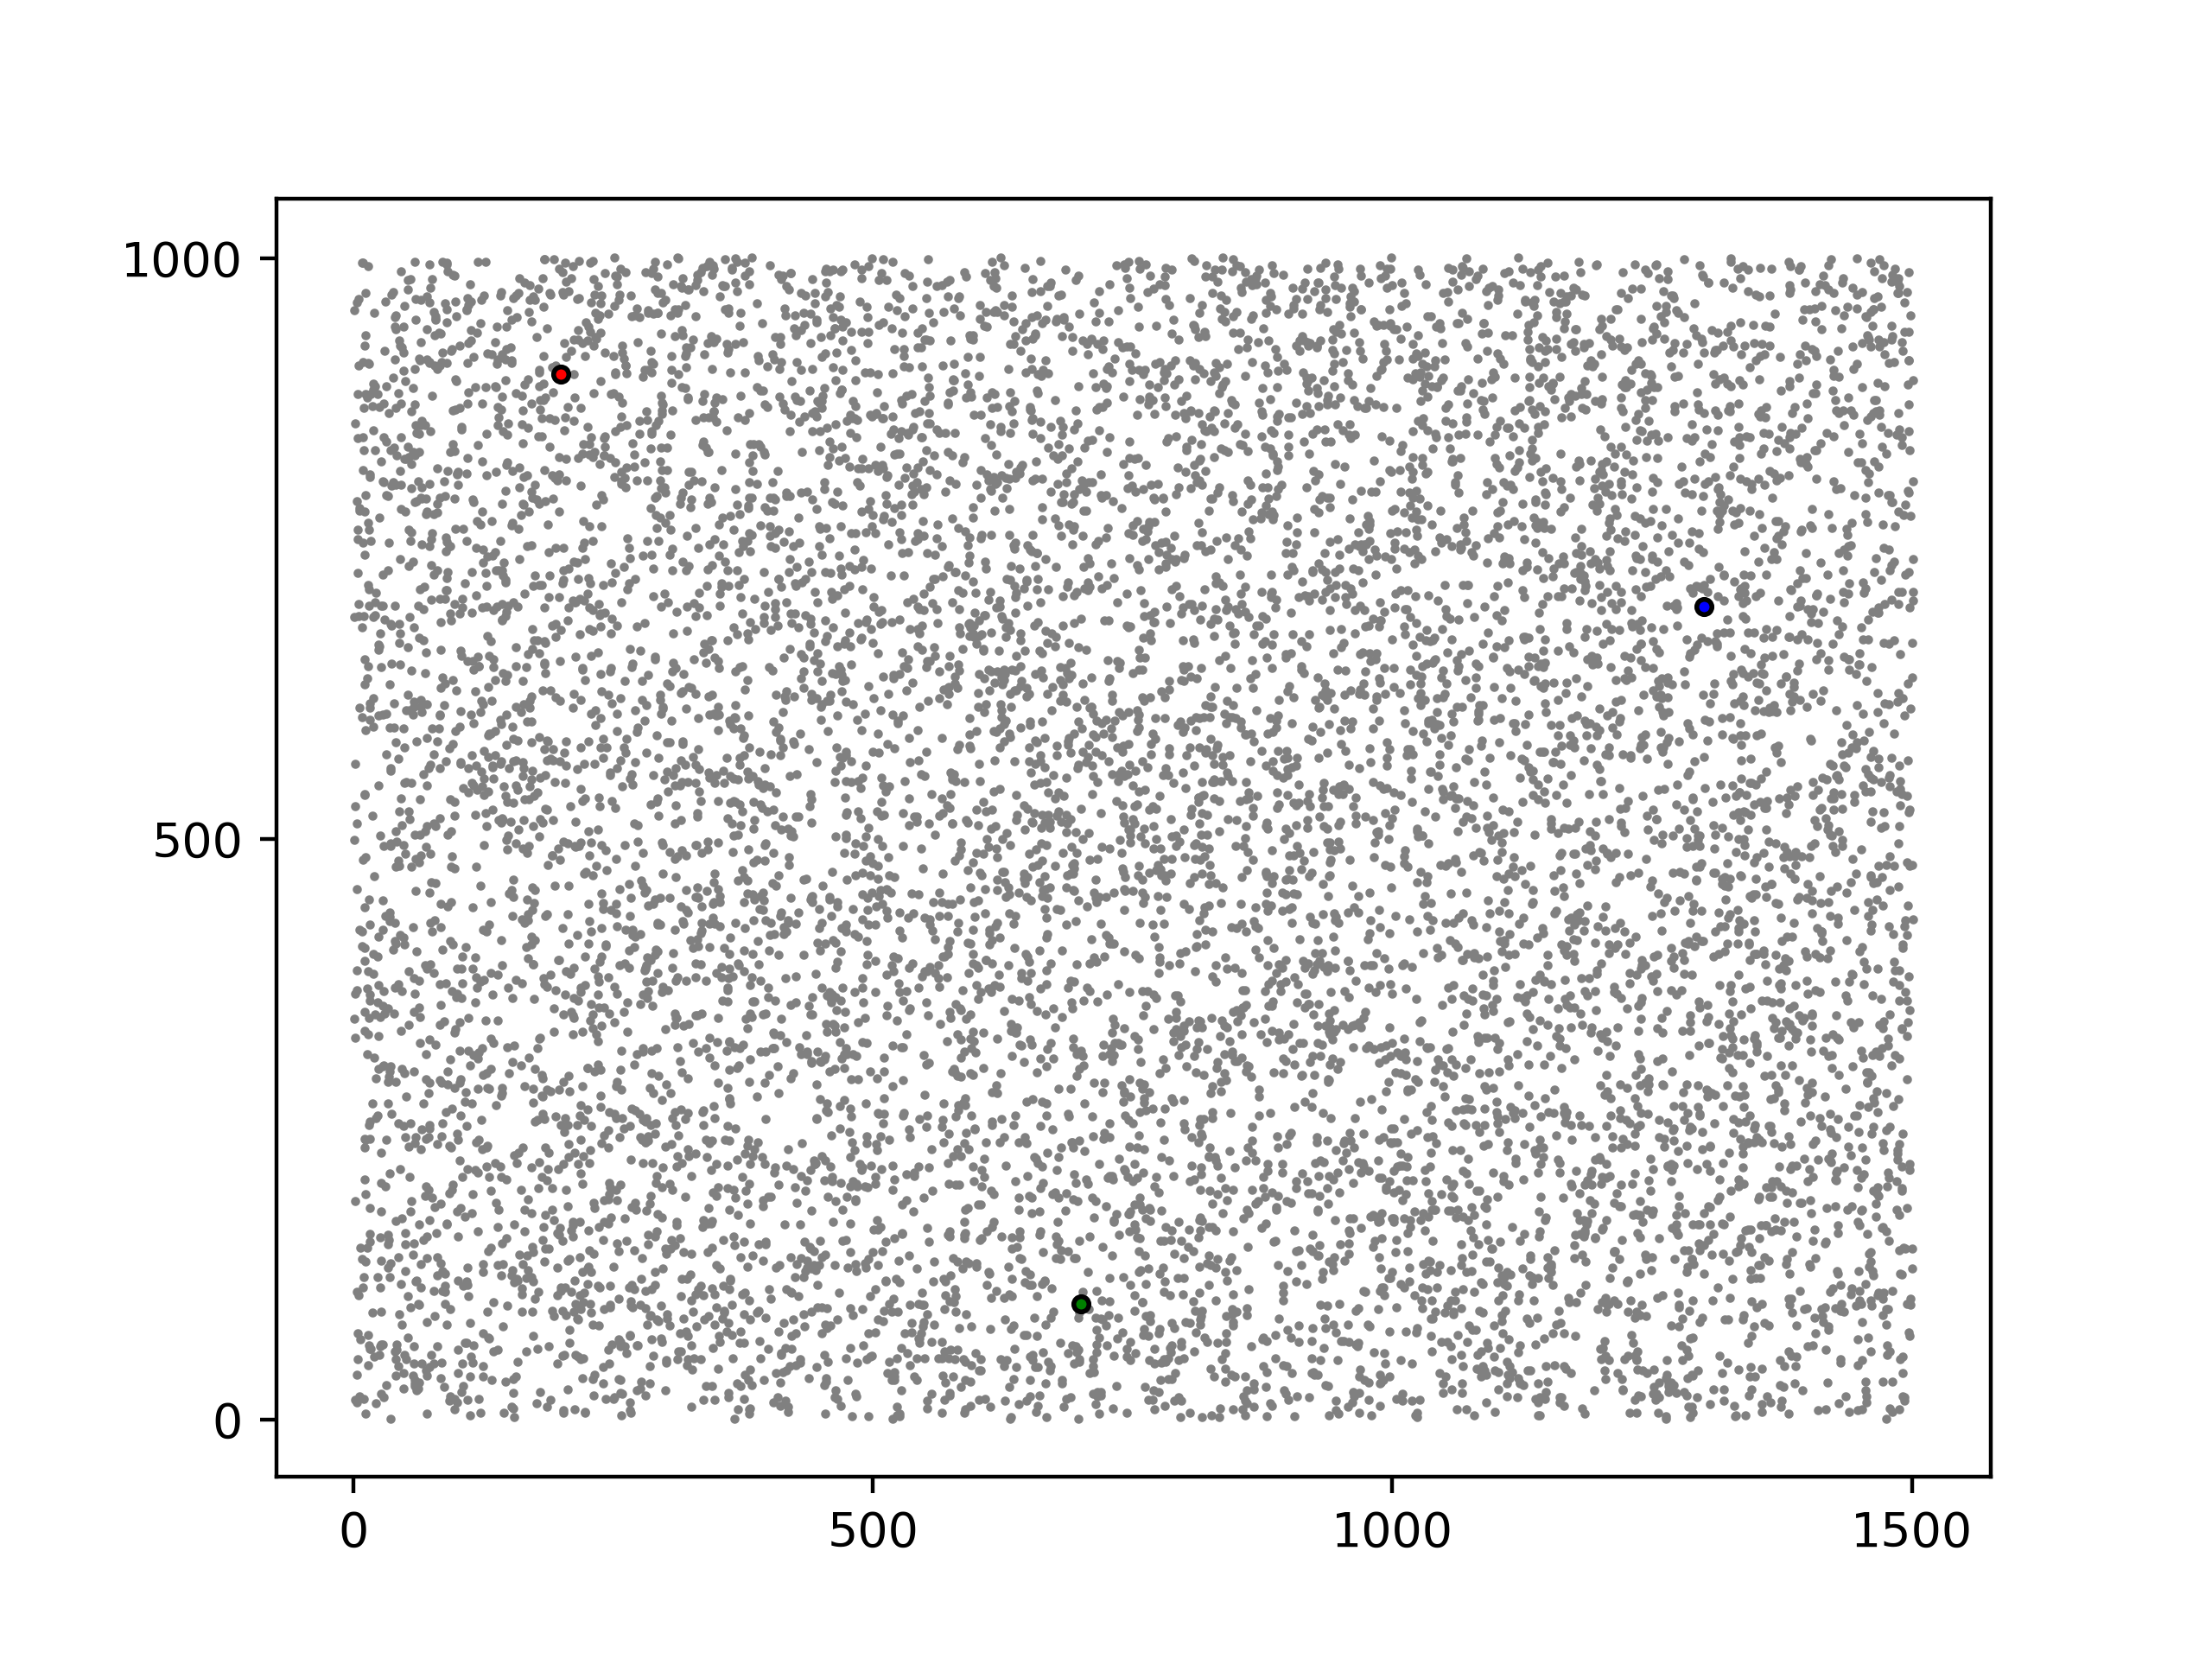
\includegraphics[width=\linewidth]{document/chapters/chapter_6/images/computation_start.png}
    \caption{Computation - Starting point}
    \label{fig:computation_start}
\end{figure}

\textbf{Given a Cartesian plane} (width: [0,1500], height: [0, 1000]) \textbf{and a set of 2D points} contained in it, \textbf{the map function takes as input one of said points and calculates the euclidean distance from each one of the centroids}; the centroid with \textbf{minimum distance among the three is then chosen, obtaining a key-value output} composed by the chosen class as the key and an array containing the computed point as the value (the array becomes relevant in the reduce function). It is important to note that, in comparing the distance among two points, the square root characterizing the euclidean distance is not needed and, therefore, it is not calculated in the map function.

\begin{lstlisting}[caption={Map function},captionpos=b]
const mapFunction = (p) => {
    const x = p[0];
    const y = p[1];
    const red = Math.pow(x - 200, 2) + Math.pow(y - 900, 2);
    const green = Math.pow(x - 700, 2) + Math.pow(y - 100, 2);
    const blue = Math.pow(x - 1300, 2) + Math.pow(y - 700, 2);
    switch(Math.min(red, green, blue)){
        case red: return ["red", [p]];
        case green: return ["green", [p]];
        case blue: return ["blue", [p]];
    }
}
\end{lstlisting}

Every data region is computed by the Map Workers and, \textbf{after every point in a particular region is classified, the output} (visualized in \textit{figure \ref{fig:computation_region_computation}}) \textbf{can be computed in the reduce function which simply reunites the intermediate results with the same key} (hence belonging to the same class) in a single array.

\begin{lstlisting}[caption={Reduce function},captionpos=b]
const reduceFunction = (p1, p2) => {
    p1.push(p2[0]);
    return p1;
}
\end{lstlisting}

\begin{figure}[!ht]
    \centering
    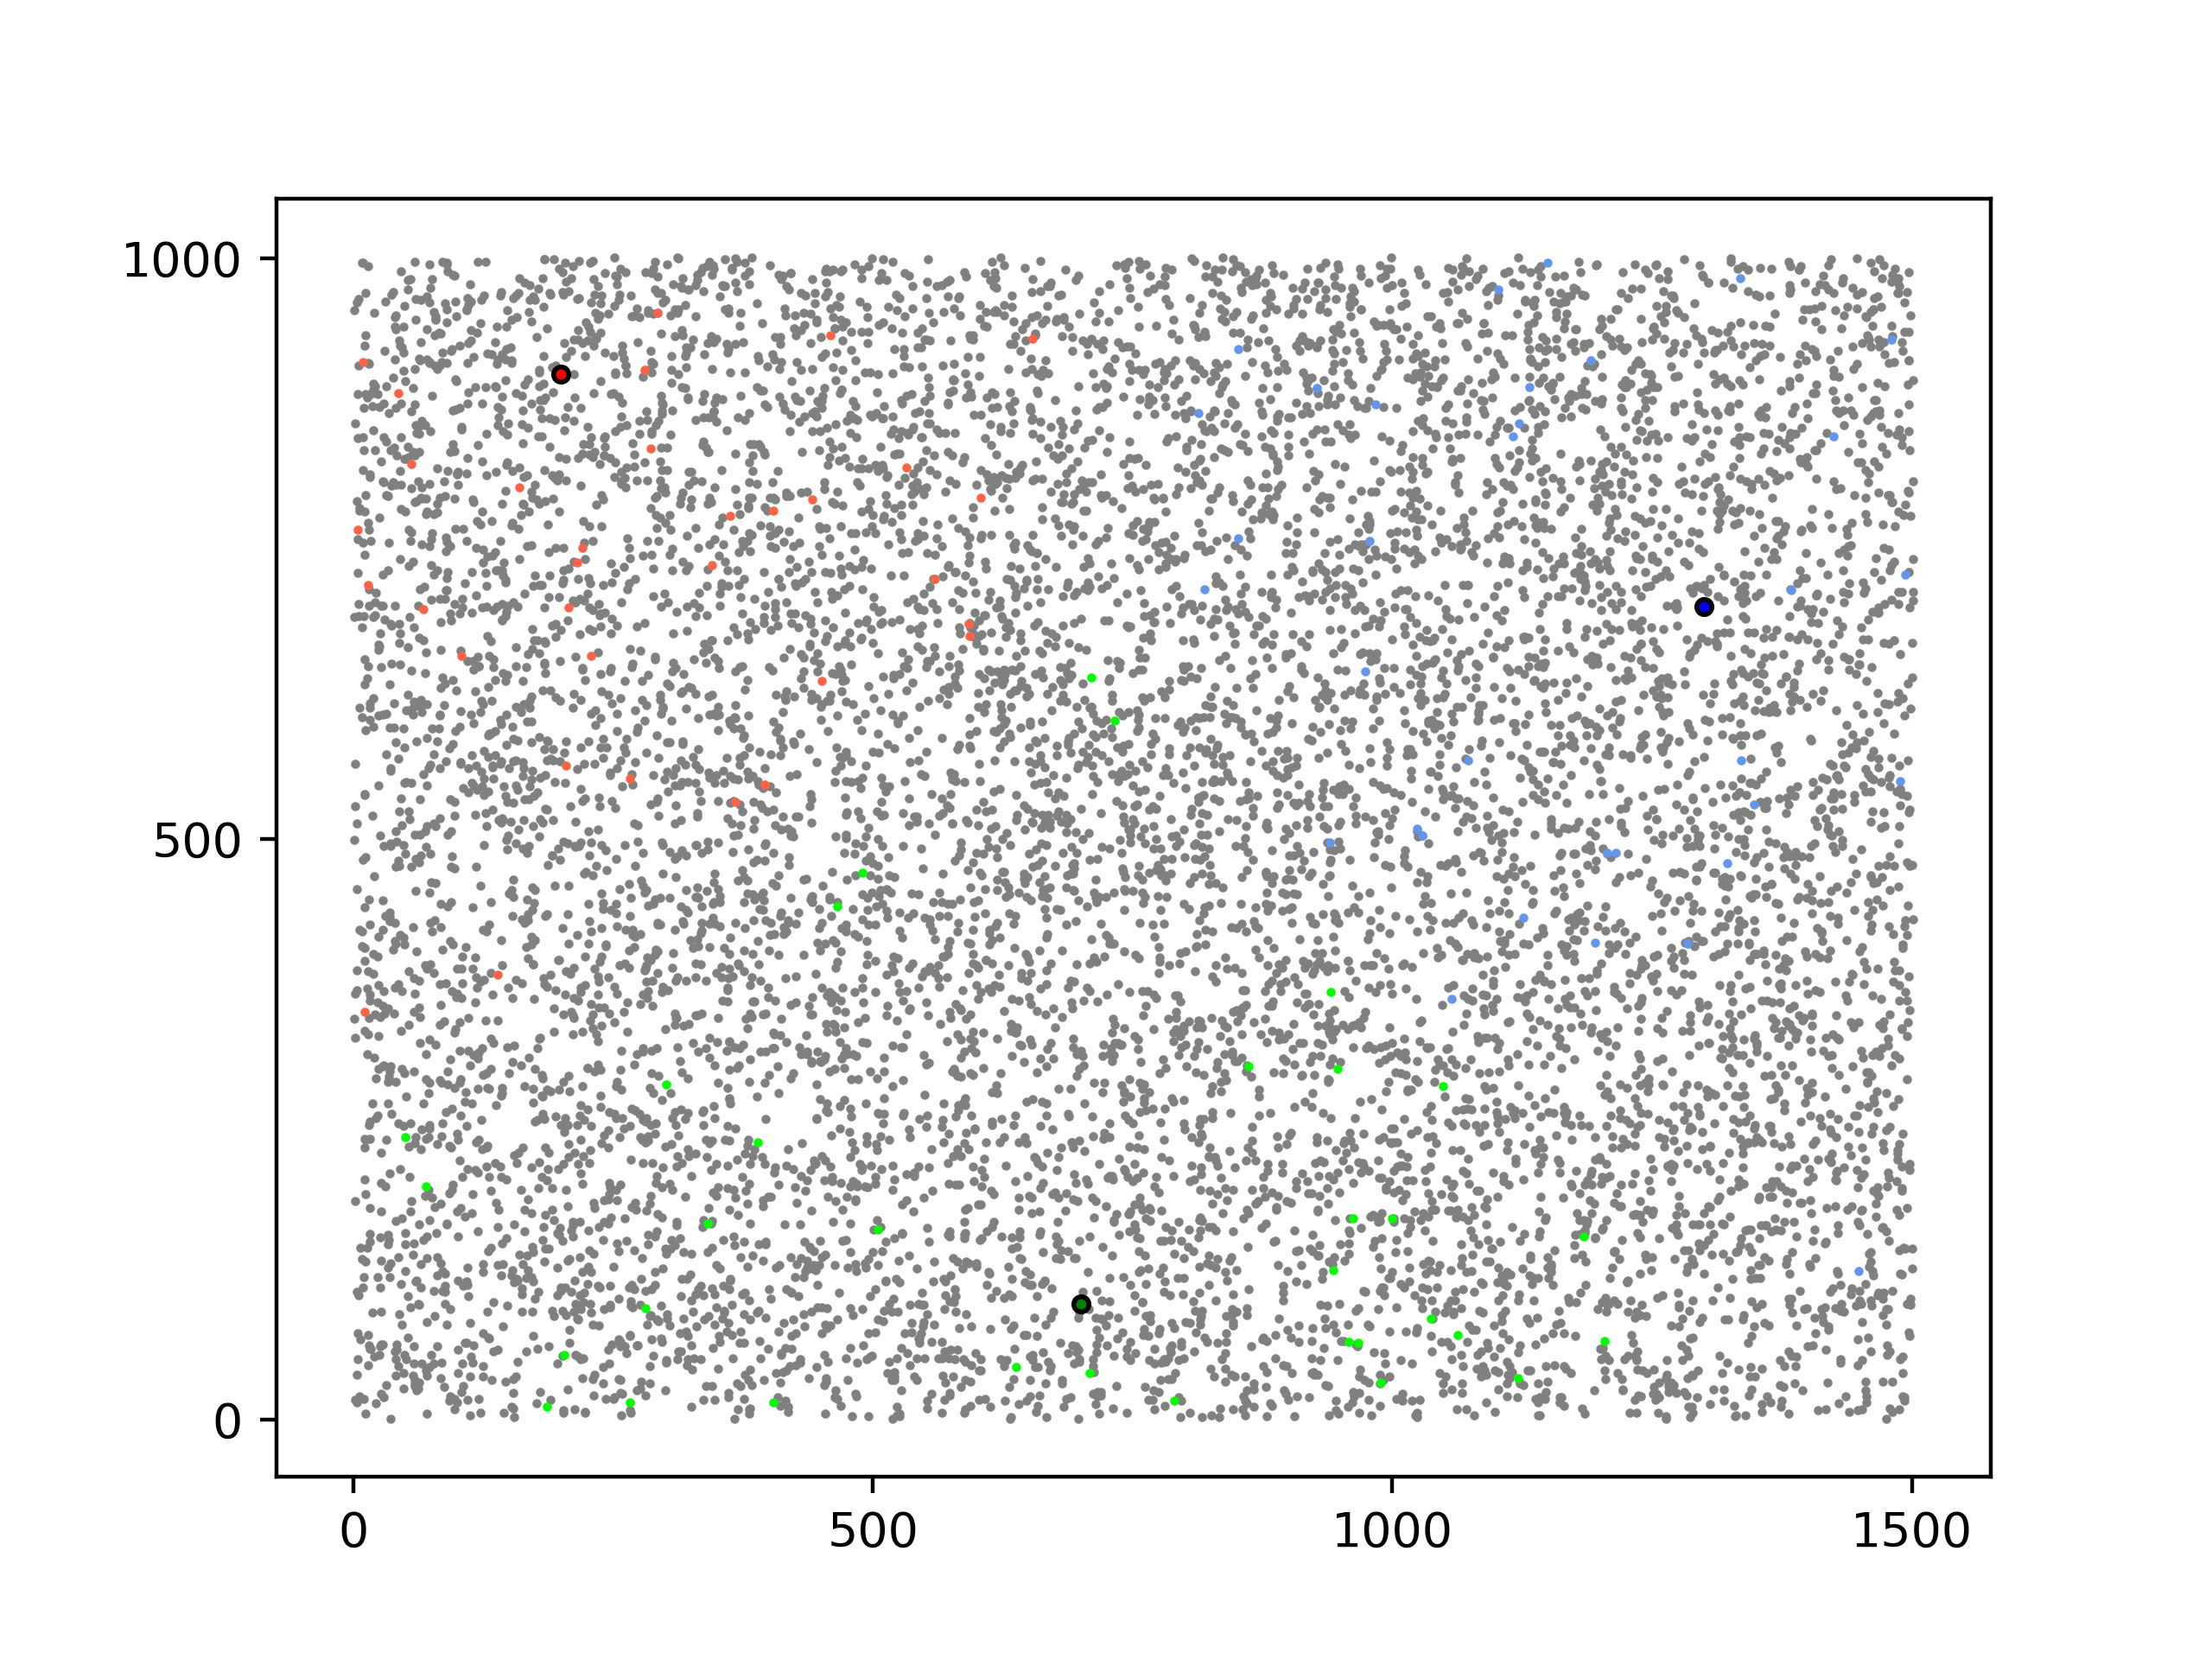
\includegraphics[width=\linewidth]{document/chapters/chapter_6/images/computation_region_computation.png}
    \caption{Computation - Region computation}
    \label{fig:computation_region_computation}
\end{figure}

As can be seen in \textit{figure \ref{fig:computation_final_result}}, after every region is mapped and then reduced, \textbf{each point is assigned to one of the three classes}.

\begin{figure}[!ht]
    \centering
    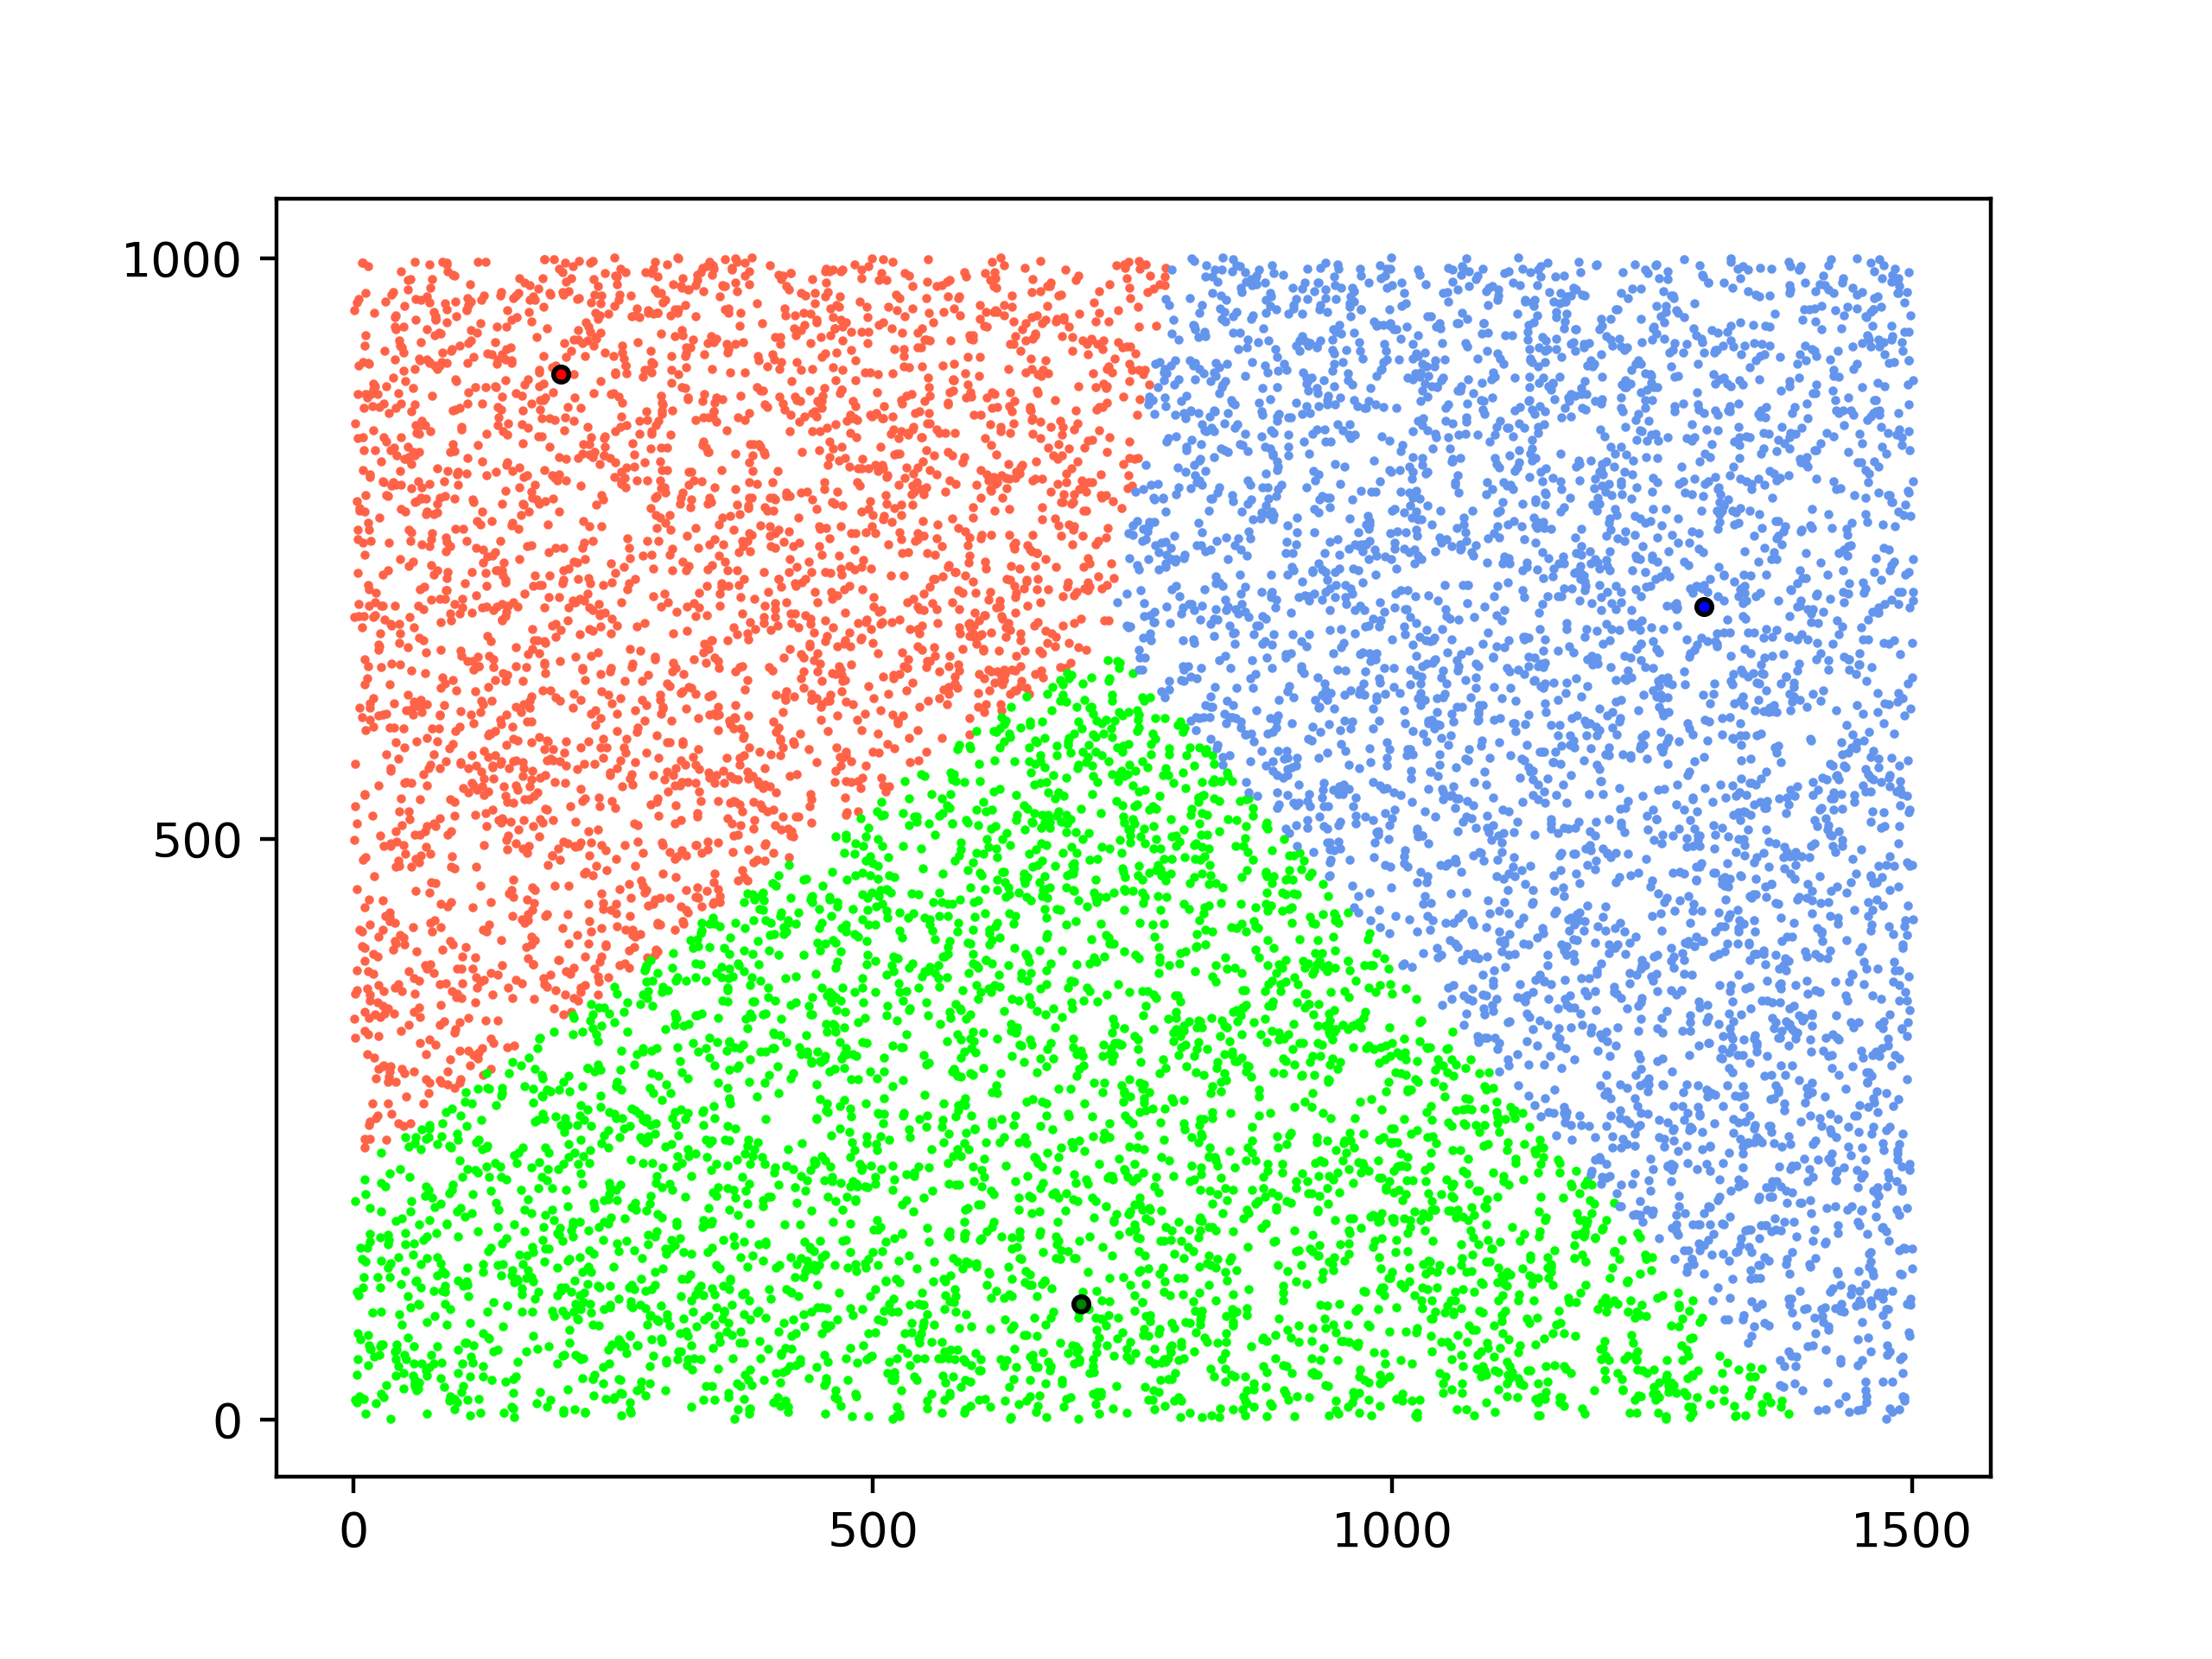
\includegraphics[width=\linewidth]{document/chapters/chapter_6/images/computation_final_result.png}
    \caption{Computation - Final result}
    \label{fig:computation_final_result}
\end{figure}

\textbf{Five experiments} were performed:
\begin{itemize}
    \item \textbf{1000 values} (10 regions, 100 points for each region)
    \item \textbf{10000 values} (100 regions, 100 points for each region)(shown in \textit{figure \ref{fig:computation_final_result}})
    \item \textbf{100000 values} (100 regions, 1000 points for each region)
    \item \textbf{1000000 values} (1000 regions, 1000 points for each region)
    \item \textbf{5000000 values} (2000 regions, 2500 points for reach region)
\end{itemize}

\subsection{Setup}
The experiment was performed in a controlled environment, meaning that only these devices were connected to the Grid (\textit{figure \ref{fig:experiment_devices_setup}}):
\begin{itemize}
    \item \textbf{A}: 1 smartphone
    \item \textbf{B}: 1 smartphone
    \item \textbf{C}: 1 computer
    \item \textbf{D}: 2 smartphones
    \item \textbf{E}: 1 tablet and 1 computer
\end{itemize}

\begin{figure}[!ht]
    \centering
    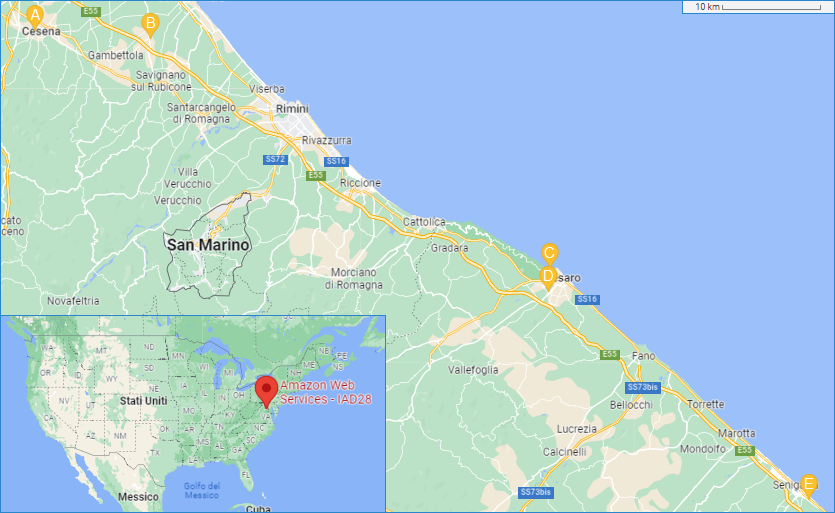
\includegraphics[width=\linewidth]{document/chapters/chapter_6/images/experiment_devices_setup.png}
    \caption{Devices setup}
    \label{fig:experiment_devices_setup}
\end{figure}

The setup of Contributing Endpoints was thus composed by \textbf{2 Interconnected Desktop Clients} and \textbf{5 Interconnected Mobile Clients}, placed in a \textbf{100 km range} in central Italy, which were forcibly chosen isolating them in a dedicated American server in order to perform multiple experiments with the same setup.

\textbf{The Invoking Endpoint Prototype instance was placed in the E location} (although it was not executed in the same computer which ran the Interconnected Desktop Client); said Invoking Endpoint requested the following resources for executing the MapReduce computation:
\begin{itemize}
    \item \textbf{4 Map Workers}
    \item \textbf{2 Reduce Workers}
\end{itemize}
    \textbf{Including the implicit MapReduce Master} (which will be taken by one of the two computers), \textbf{this adds up to the 7 devices specified earlier}, which were used in each of the five experiments.

\subsection{Results}
\textit{Figure \ref{fig:experiment_results}} shows the \textbf{results for the five experiments performed}, focusing on the \textbf{total time} and the \textbf{average time taken by each value} (both \textbf{measured in milliseconds}). Once again, these results were obtained using a very small pool of devices and the simplified nature of the MapReduce algorithm in this prototype significantly slows down the whole process (primarily because the intermediate results are first sent back to the MapReduce Master that then forwards them to the Reduce Worker, instead using a direct connection among Map Worker and Reduce Worker).

\begin{figure}[!ht]
    \centering
    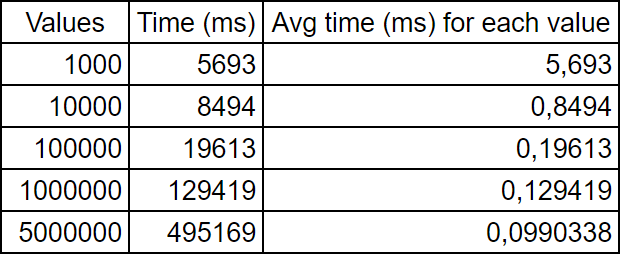
\includegraphics[scale=0.55]{document/chapters/chapter_6/images/experiment_results.png}
    \caption{Experiment results}
    \label{fig:experiment_results}
\end{figure}

The \textbf{first significant observation} can be made l\textbf{ooking at the first two experiments}: the \textbf{average time for each value drastically drops} (\texttildelow6.7 times faster); this can be \textbf{explained by considering that the total time also includes the recruitment phase where no computation is executed}. In other terms, \textbf{the number of values used in the first experiment is so small that their computation time becomes irrelevant}, meaning that the recruitment phase is basically the only factor that influences the average time. \textbf{The more values are computed (assuming the same number of devices are used), the less impactful the recruitment time becomes}.

\begin{figure}[!ht]
    \centering
    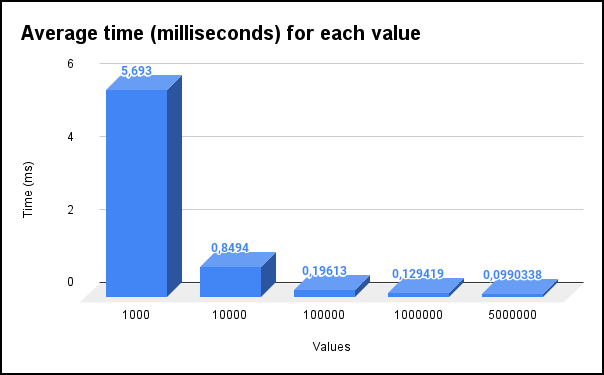
\includegraphics[scale=0.55]{document/chapters/chapter_6/images/experiment_results_avg_ms_per_value.png}
    \caption{Average time (milliseconds) for each value}
    \label{fig:experiment_results_avg_ms_per_value}
\end{figure}

Finally, \textit{figure \ref{fig:experiment_results_avg_ms_per_value}} focuses on \textbf{comparing the average time for each value}; it becomes apparent that, despite the not optimized algorithms used in this prototype, \textbf{the more values are computed, the greater the advantage becomes, showing that a distributed computation participated also by mobile devices is not only feasible, but it can also provide value to the Customer}.
